\documentclass[12pt]{support/thcolognethesis} 

\usepackage{amssymb}

\title{Optimierung von Augmented Reality Anwendungen durch die Berücksichtigung von Tiefeninformationen mit Googles Project Tango}

\degree{Masterthesis}

\author{Steffen Tröster}

\college{
	Technischen Hochschule Köln\\
    Ingenieurwissenschaftliches Zentrum\\
    Fakultät für Informations-,\\
    Medien- und Elektrotechnik}

\course{Technische Informatik (Master)}

\company{inovex GmbH}  

\firstExaminer{Prof. Dr. Hubert Randerath}
\firstExaminerLocation{Technische Hochschule Köln}
\secondExaminer{Prof. Dr. Martin Eisemann}
\secondExaminerLocation{Technische Hochschule Köln}

\degreedate{Köln, im \monthyeardate\today}
	
\begin{document}

\baselineskip=18pt plus1pt

\setcounter{secnumdepth}{3}
\setcounter{tocdepth}{3}

\maketitle                 

\begin{abstract}
\setlength{\parskip}{1em}

Project Tango ist eine neue mobile Plattform des Google Advanced Technology and Project (ATAP) Teams, die in der Lage ist, Bewegungsverfolgung, Tiefenwahrnehmung und Umgebungswiedererkennung auf Smartphones und Tablets anbieten zu können. Durch die kontinuierliche Bestimmung der relativen Geräteposition eignet sich die Plattform besonders für dreidimensionale Augmented Reality (AR) Anwendungen. Die Illusion dieser AR Anwendungen wird besonders dann gestört, wenn sich reale Objekte in einer Szene räumlich vor virtuellen Objekten befindet und diese virtuellen Objekte nicht entsprechend ausgespart werden. 

Diese Arbeit stellt daher drei Überdeckungsverfahren vor, mit denen diese Überlagerung der virtuellen Objekte mit Hilfe der Tiefenwahrnehmung von Project Tango und des Z-Buffer Algorithmus realisiert werden kann. Die Tiefeninformationen für den Z-Buffer werden hierfür zum einen direkt aus den Sensordaten und alternativ mit einer TSDF Rekonstruktion und einer selbst zusammengestellten Ebenen Rekonstruktion bestimmt. Außerdem wird auf einen zusätzlichen Ansatz eingegangen, der zur Verbesserung dieser Tiefeninformationen die Bildinformationen der Farbkamera durch den Guided Filter berücksichtigt. Diese Mechanismen werden im Laufe der Arbeit prototypisch umgesetzt und gegenübergestellt. 

\setlength{\parskip}{0em}
\end{abstract}
\selectlanguage{english}
\begin{abstract}
\setlength{\parskip}{1em}

Project Tango is a new mobile platform by Google’s Advanced Technology and Projects (ATAP) Teams, which brings Motion Tracking, Depth Perception, and Area Learning to mobile devices. With Project Tango, Google is providing a technology to tablets and smartphones for building virtual reality (VR), indoor navigation, precise measurement and augmented reality applications. The focus of this document lies mainly upon augmented reality applications. Although you can build an effective 3D AR illusion with the continuous device motion tracking, there is still a problem, that the scenes virtual object cannot be occluded by real objects when they are in foreground.

Since the Project Tango platform is offering a continues depth perception of the current viewport, this depth information can be used to solve the missing occlusion issue. This work is introducing three approaches to enable an augmented reality occlusion by real objects. Additionally an approach will be discussed to optimize the depth occlusion by taking the color information by the device’s camera into account. These methods will also get implemented with the development kit, tested, compared and evaluated concerning their applicability.

\setlength{\parskip}{0em}
\end{abstract}
\selectlanguage{ngerman}


         

\begin{romanpages}         
\tableofcontents            
\end{romanpages}          

% Einleitung
\chapter{Einleitung}

Project Tango ist eine neue mobile Plattform des Google Advanced Technology and Projects (ATAP) Teams, welche Bewegungsverfolgung, Tiefenwahrnehmung und Umgebungswiedererkennung auf mobilen Endgeräten realisiert.

\begin{quotation}
\enquote{Project Tango combines 3D motion tracking with depth sensing to give your mobile device the ability to know where it is and how it moves through space.}  \citep{Proje19:online}
\end{quotation}

Diese Verfügbarkeit dieser Echtzeitdaten ermöglicht viele verschiedene neue Einsatzmöglichkeiten auf mobilen Endgeräten wie Smartphones und Tablets. Typische Einsatzszenarien dieser Plattform sind die Indoor Navigation, die Vermessung der Umgebung sowie andere Anwendungen im Bereich Virtual und Augmented Reality. Der Fokus dieser Forschungsarbeit liegt hier in dem Anwendungsbereich der dreidimensionalen Augmented Reality (AR). 

Die Anwendungsgebiete für Augmented Reality (dt. Erweiterte Realität) sind sehr vielseitig und liegen in der Medizin, der Unterhaltungsindustrie, Bildung und in vielen weiteren Industriezweigen. Eine barrierefreie Navigationshilfe, Einblendungen für die persönliche Assistenz, kontextsensitive Projektionen und Computerspiele sind Beispiele für typische Anwendungen, die durch AR umgesetzt werden können. 

Für die erfolgreiche Umsetzen einer Augmented Reality Anwendung, müssen die Kameraeigenschaften, wie Brennweite, Verzerrung und die Position der Kamera zu jeder Zeit und idealerweise in Echtzeit bekannt sein. Sensoren wie Kompass, INS (Trägheits\-navigations\-system) oder GPS können zwar eine grobe Lokalisierung ohne bekannte Merkmale im Raum ermöglichen, führen aber langfristig zu Fehlern, wenn keine optischen Referenzen gegeben sind. Mit Hilfe von der Bewegungsverfolgung durch Project Tango kann diese Lokalisierung der Kamera und somit die korrekte Positionierung von virtuellen Objekten im Raum deutlich zuverlässiger, in Echtzeit und ohne vordefinierte Merkmale im Raum realisiert werden. Project Tango eignet sich daher sehr gut für die Umsetzung und den Einsatz von AR Anwendungen.

\section{Augmented Reality Optimierung}

Um eine für den Betrachter effektive und optimierte Augmented Reality Anwendung umsetzen zu können, benötigt man laut \citet{azuma2001recent} die Möglichkeit mehr Informationen über relevante Objekte im realen Raum ermitteln zu können. Durch diese Informationen könnte dem Nutzer zum Beispiel eine Interaktion mit realen Objekten ermöglicht werden oder anhand optischer und semantischer Einordnung der Umgebung passende Funktionen angeboten werden. 

Hinsichtlich der zuletzt erwähnten Kontextsensitivität existieren viele Ansätze, basierend auf optischen Merkmalen der Umgebung. So kann zum Beispiel ein optisches Tracking von realen Objekten, wie von \citet{lee2008hybrid} beschrieben, umgesetzt werden. Project Tango nutzt bereits optische Merkmale, um eine Positionsverfolgung oder das Lernen der Umgebung umzusetzen. Wären diese Merkmale für den Entwickler als Schnittstelle verfügbar, könnte man mit diesen Informationen solche kontextsensitiven Anwendungen umsetzen. Der Fokus soll in dieser Arbeit jedoch nicht auf den optischen Merkmalen sondern auf den Tiefeninformationen, die Project Tango durch den eingebauten Tiefensensor in Form einer Pointcloud liefern kann, liegen.

Ein sinnvoller Einsatz von Augmented Reality Anwendungen besteht darin, virtuelle Objekte in eine echte Szene zu projizieren. Dabei überlagert die Projektion des virtuellen Objekts das aktuelle Kamerabild oder den aktuellen Sichtbereich und erwirkt dadurch den Anschein, als ob sich das virtuelle Objekt wirklich in der Szene befindet. Dieser Effekt funktioniert solange erfolgreich, bis ein reales Objekt sich räumlich vor das virtuelle Objekt bewegt und die zu erwartende Überlagerung des virtuellen Objekts nicht erfolgt. Diese fehlerhafte Darstellung durch eine fehlende Überdeckung ist in Abbildung \ref{fig:occlusion-problem} zu erkennen. 

\begin{figure}[h]
  \centering
	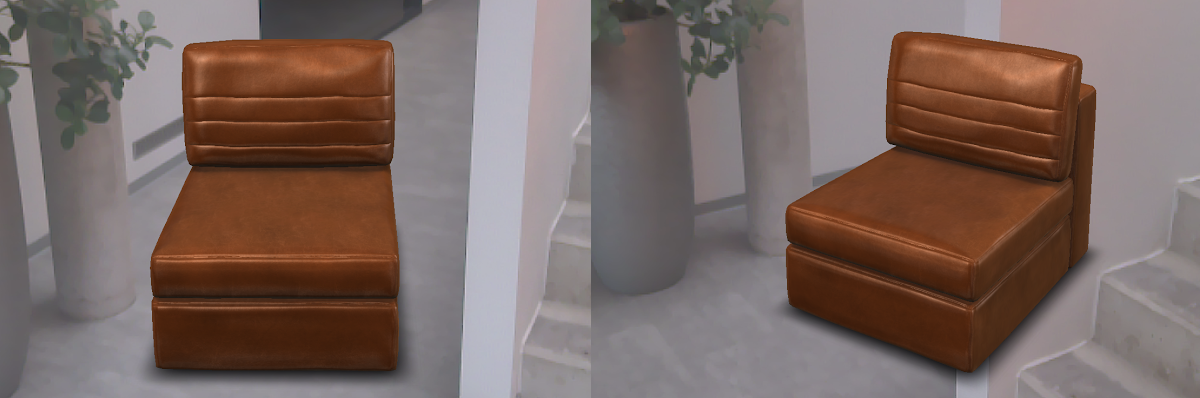
\includegraphics[width=1.0\textwidth]{content/images/occlusion-problem.png} 

  \caption{AR Projektion mit Project Tango - Links: Erfolgreiche Projektion. Rechts: Fehlerhafte Darstellung ohne Überdeckung.}
  \label{fig:occlusion-problem}
\end{figure}

Die Verfügbarkeit der Tiefeninformationen bei Project Tango könnte die Interaktionen oder Darstellungen in einer Augmented Reality Anwendung präziser an die echten räumlichen Gegebenheiten anpassen. Es existieren zum Beispiel prototypische Anwendungen, in denen virtuelle Markierungen passend an echten Objekten im virtuellen Raum positioniert werden können, indem sie auf die aktuellen Tiefeninformation des Sichtbereichs zurückgreifen. Eine weitere Idee ist es, Überlagerungen virtueller Objekte ermitteln zu können, an denen sich reale Objekte im Vordergrund befinden.

\section{Zielsetzung und Vorgehen}

Diese Arbeit will die Fragestellung beantworten, durch welche Verfahren mithilfe der Tiefeninformationen von Project Tango, automatisch und in Echtzeit die Überdeckung virtueller Objekte mit realen Objekten in einer Augmented Reality Szene realisiert werden kann. Dabei soll Project Tango als autonomes System betrachtet werden, welches diese Problemstellung selbstständig und mit den eingeschränkten Ressourcen dieser mobilen Plattform lösen soll.

Hierzu sollen zunächst bestehende Verfahren zur Bestimmung einer Augmented Reality Überdeckung durch eine Literaturrecherche gefunden werden. Diese Verfahren sollen dabei auf Ihre Anwendbarkeit mit der Project Tango Hardware überprüft werden. Sollten sich aus der Recherche weitere Ideen ergeben, wie speziell auf der Project Tango Hardware eine Überdeckung umgesetzt oder verbessert werden kann, sollen diese mit in die Arbeit eingebunden werden. Eine Idee könnte zum Beispiel sein, auch das Farbbild der normalen Kamera von Project Tango in die Optimierung der virtuellen Überlagerung einfließen zu lassen. Die identifizierten Verfahren sollen hiernach entsprechend implementiert werden, um sie darauf folgend in einer Testumgebung gegenüber zu stellen.

Strukturell wird in dieser Arbeit in Kapitel \ref{sec:thema} erst einmal auf die thematischen Grundlagen zu Augmented Reality und Project Tango eingegangen. Hier werden auch die existierenden Verfahren zur AR Überdeckung angesprochen. Unter Kapitel \ref{sec:algorithms} sind theoretische Grundlagen zu finden, die bei der späteren Umsetzung verschiedener Verfahren angewendet werden. Kapitel \ref{sec:optimization} beinhaltet die Argumentation und Beschreibung der gewählten Verfahren, welche unter Kapitel \ref{sec:implementation} auf der Project Tango Hardware umgesetzt werden. In Kapitel \ref{sec:evaluation} werden die vorliegenden Umsetzung in einem Testszenario gegenübergestellt, um eine Aussage treffen zu können, welcher Ansatz auf der Hardware oder für einen bestimmten Einsatz gut funktionieren könnte.




% Thematische Vorbemerkung
\chapter{Thematische Vorbemerkung}

Im ersten Teil dieses Kapitels werden zunächst einmal die Grundlagen zu Augmented Reality beschrieben, wie diese Technologie einzuordnen ist, welche technischen Anforderungen ein Augmented Reality System hat und wo typische Einsatzszenarien liegen. Hiernach wird näher auf Googles Project Tango eingegangen, welche Konzepte angewendet werden und wie diese Technologie im Bereich Augmented Reality einzuordnen ist. \\


\section{Augmented Reality}

Augmented Reality (AR) ist eine Klasse aus dem Realitäts-Virtualitäts-Kontinuum von \cite{milgram1995augmented}, welches in Abbildung \ref{fig:virtual-continuum} abgebildet ist. Diese Klasse beschreibt die Darstellungen von realen und virtuellen Informationen in einer Repräsentationsform, wobei hier reale und virtuelle Objekte in einer realen Umgebung kombiniert dargestellt werden können. Diese virtuellen Objekte sind in der realen Umgebung idealerweise fest lokalisiert und fügen sich somit in das reale Erscheinungsbild ein. Typischerweise sind AR Anwendungen interaktiv, und stellen die virtuellen Objekte in Echtzeit und dreidimensional in der realen Welt dar. Für die Definition von AR Anwendungen gibt es zudem keine Limitierung für die Darstellungstechnologie, wie zum Beispiel das Projekt Tango Tablett oder einem Head-Mounted Display. AR beschränkt sich zudem nicht auf den angesprochenen Sinn - so sind zum Beispiel AR Anwendungen mit visueller, taktiler oder sogar olfaktorischer Umsetzung möglich.\\

\begin{figure}
  \centering
	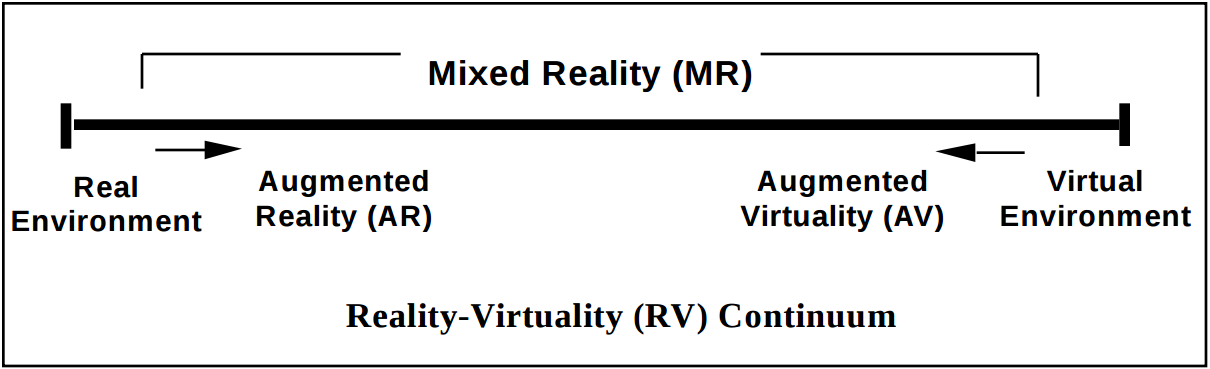
\includegraphics[width=0.85\textwidth]{content/images/theory/virtual-continuum.png} 
  \caption{Vereinfachte Darstellung des Realitäts-Virtualitäts-Kontinuum von \citet*{milgram1995augmented}}
  \label{fig:virtual-continuum}
\end{figure}


Virtuel Reality (VR) oder auch Virtual Environment hingegen kapselt sich von der realen Umgebung ab und bietet Interaktionen in reinen virtuellen Umgebungen. Diese rein virtuelle Darstellung konnte sich im Gegensatz zu Augmented Reality deutlich schneller Entwickeln, da die technologischen Anforderungen an AR deutlich höher sind. \citep{van2010survey}\\

\subsection{Technische Anforderungen}

Dieser Abschnitt widmet sich den technischen Anforderungen an Augmented Reality, indem die potentiellen Display Technologien beschrieben werden, mögliche Trackingverfahren zur Ermittlung der Betrachtungsposition erläutern werden und auch die Systeme behandelt werden, mit denen ein Nutzer mit den virtuellen Darstellungen interagieren kann.\\

\subsubsection{Display Technologie}

Der erste wichtige Teil der technologischen Anforderungen an AR sind visuelle Anzeigen (visual displays), die neben der Möglichkeit eines dreidimensionalen Renderings, welches hier aus der Virtual Reality vorausgesetzt werden soll, weitere Charakteristika mit sich bringen. Nach \citet{van2010survey} lassen sich diese Technologien zunächst in je drei Arten der Darstellung und Positionierung unterteilen.  \\

Die einfachste und günstigste Art der visuellen Darstellung in AR ist \enquote{video see-through}, wodurch die reale Umgebung durch eine Video Aufnahme ersetzt wird und die virtuellen Objekte digital in die Video Aufnahme gerendert werden. Das bietet die Möglichkeit Objekte aus der realen Umgebung zu entfernen oder zu ändern oder, anhand der Luminanz Information vom Video, das Rendering der virtuellen Objekte entsprechend an die Realität anzupassen. Anwendung findet diese Technologie typischerweise in Tablets oder Smartphones.\\

Die nächste Möglichkeit zur Darstellung ist \enquote{optical see-through}. Hier werden die virtuellen Objekte durch transparente Spiegel in das Sichtfeld des Betrachters gebracht. Anders als bei \enquote{video see-throught} bleibt die reale Auflösung für die visuelle Aufnahme des Betrachtes gleich und es können zudem keine Latenzprobleme beim Ändern des Betrachtungswinkels auftreten (parallax-effect). Auf der anderen Seite besteht bei dieser Technologie das Problem, dass die Darstellung von virtuellen Objekten nicht kräftig genug ist, um die reale Umgebung auf Grund von der transparenten Darstellungsoberfläche komplett auszublenden. Typische Geräte dieser Technologie sind Headmounted Displays wie Google Glass oder stationäre Geräte wie der HoloDesk.\\

Die dritte Möglichkeit ist die projizierte Darstellung, in der die Augmented Reality Überlagerung auf die realen Objekte projiziert werden. Diese Darstellung ermöglicht die Abdeckung vom gesamten Sichtfeld des Betrachters, benötigt aber eine entsprechende Kalibrierung oder eine Strukturwahrnehmung bei Umgebungsänderungen.\\

Neben der Art der Darstellung können die Display Technologien laut \citet{azuma2001recent} anhand Ihrer Positionierung klassifiziert werden. Man unterscheidet zwischen am Kopf befestigten Displays (head-mounted), tragbaren Displays (hand-held) und räumlich positionierten Displays. Zu jeder dieser Displayarten gibt es wiederum unterschiedliche technische Umsetzungen mit ihren spezifischen Vor- und Nachteilen bezüglich ihrer Anwendungsszenarien.\\

\subsubsection{Tracking Technologien}

Um eine virtuelle Projektion im realen Raum auf nicht stationären Displaytechnologien zu realisieren muss die Position und gegebenenfalls relative Positionsänderung des Displays bestimmt werden, auch \enquote{augmented reality registration} genannt. Man spricht dabei üblichweise von den \enquote{six degrees of freedom (6DOF)}, der Position im Raum (x, y, z) und der Orientierung (yaw, pitch, roll). \\

Frühe Techniken für die Registrierung benötigten üblicher Weise eine speziell vorbereitete Räumlichkeit, denn sie basierten auf mechanischen, magnetischen oder Ultraschall Sensoren um die Position zu bestimmen. Diese Sensoren sind zwar immer noch im Einsatz und bilden auch den Grundstein für die AR und VR Forschung, sind aber praktisch gesehen zu komplex und aufwändig für die meisten Anwendungsfälle. \citep{van2010survey} \\

Für ein grobes Positions-Tracking, vor allem auch außerhalb von Gebäuden wird GPS genutzt. Für großräumliche Anwendung ist GPS, mit einer Varianz von 10-15 Metern und in Kombination mit einem Kompass, durchaus praktikabel. Zum Beispiel um sichtbare Flugzeuge oder Sterne visuell aufzubereiten. Innerhalb von Gebäuden basiert die grobe Positionierung laut \citet{van2010survey} oft auf verfügbaren Wifi Access Points oder RFID Markern. \citet{lamarca2005place} demonstrieren hierzu auch die Möglichkeit diese Idee für grobe Lokalisation außerhalb von Gebäuden einzusetzen.\\

Optische Tracking Verfahren basierend auf Bildverarbeitung bieten laut \citet{van2010survey} deutlich genauere Resultate als die zuvor beschriebenen Verfahren. Es gibt hier viele verschiedene sensorische Ansätze ein optisches Tracking zu realisieren. Frühe verfahren nutzten referenzielle Marker oder Licht emittierende LEDs in einem vordefinierten Modell, um zwischen aufgenommenen Bildern eine homographische Transformation zu berechnen und um somit Rückschlüsse auf die Rotation und Positionsänderung der Kamera zu ziehen. Neue Verfahren ohne Marker, wie das sogenannte \enquote{visual odometry} von \citet{nister2004visual}, nutzen Techniken zur Feature Detection und Matching um Referenzen und Bewegungen zwischen aufgenommenen Bildern zu bestimmen.\\

Viele kommerzielle und erfolgreiche Tracking Verfahren beruhen jedoch auf hybride Ansätze, in denen die Informationen mehrerer Sensoren kombiniert werden, um potentielle Messfehler eines Sensors oder einer Methodik auszuschließen. So werden zum Beispiel Neigungssensor, Kompass und Gyroskop mit einem optischen Verfahren kombiniert, um ein Tracking der sechs Freiheitsgrade zu optimieren. Diese Erweiterung des optischen Verfahrens wird auch \enquote{visual-inertial odometry} genannt. \citep{van2010survey}\\

\citet{azuma2001recent} erwähnt an dieser Stelle auch die Kalibrierung der Sensoren, die für ein präzises Registrieren nötig ist. So müssen zum Beispiel die Linseneigenschaften der Kamera für optisches Tracking bekannt sein, damit die Verfahren mit Krümmungen, Verzerrungen und den perspektivischen Eigenschaften umgehen können. Diese Informationen sind auch bei video see-through Displays für ein korrektes Projizieren der 3D Objekte wichtig. Zudem wird erwähnt, dass man Messfehlern oder Drifts der Position zum Beispiel mit der Zunahme von Gyroscop Informationen entgegenwirken kann, indem man Ereignisse wie einen Schritt des Nutzers einfließen lässt. \citep{azuma2001recent} \\

\subsubsection{Interaktions Technologien}

Neben den Display und Tracking Technologien ist es notwendig dem Nutzer andere Interaktionsmöglichkeiten anzubieten, da in der Regel das klassische zweidimensionale WIMP Paradigma (Windows, Icons, Menus and Pointer) im dreidimensionalen Kontext von AR keine ausreichende Gebrauchstauglichkeit bietet. Dennoch müssen die Interaktionstechnologien in Augmented Reality die üblichen Interaktionen wie aus WIMP unterstützen. Dazu gehören zum Beispiel das Auswählen, Positionieren und Drehen von virtuellen Objekten, das Zeichnen von Pfaden oder Flugbahnen, sowie die Eingabe von Quantitativen Werten oder Texten. \citep{van2010survey} \\

Frühe Augmented Realilty Systeme nutzen einfache Trackballs, Trackpads, Touchscreens oder Gyroscopmäuse für eine zweidimensionale Interaktion mit dem System. Später wurden dreidimensionale Equivalente eingeführt, wie 3D Mäuse oder Stifte, die eine dreidimensionale Interaktion ermöglichen. Diese Greifbaren Schnittstellen werden auch TUIs genannt (Tangible User Interface) und ermöglichen eine unidirektionale Interaktion mit dem System. Zudem wurden auch TUIs mit haptischen Feedback eingeführt, wie zum Beispiel die 3D Maus PHANTOM. \citep{van2010survey} \\

Eine weitere Art der TUIs sind laut \citet{azuma2001recent} Gegenstände, mit denen der Nutzer natürlich interagieren kann und die vom System optisch erfasst werden, um die Positionsänderung der Objekte anhand von Markern oder anderen optischen Merkmalen zu bestimmen. Somit kann ein Nutzer, zum Beispiel, für die virtuelle Einrichtung eines Raums, die Möbel mit Hilfe eines echten Gegenstands im Raum verschieben. \\

Nicht taktile Systeme verwenden meist optische Aufnahmen um Gesten der Hände, des gesamten Körpers oder die Blickrichtung des Nutzers zu erkennen. Dabei werden Kameras am Körper oder im Raum verwendet. Außerdem ist es Möglich Spracherkennung in die Interaktion mit einfließen zu lassen, um eine möglichst authentische Interaktion zu bieten. Wie auch bei den Tracking Technologien existieren hierbei Hybride Systeme, die verschiedene Interaktions Technologien kombinieren. \citep{van2010survey} \\

\subsection{Anwendungsbereiche}

Über die Jahre habe Wissenschaftler immer mehr Bereiche identifiziert, die von der Anwendung von Augmented Reality profitieren können. \citet{van2010survey} nennt dazu als Erstes Einsatzgebiet die persönliche Assistenz, in der AR Systeme eingesetzt werden können, um zum Beispiel mit Hilfe von Brillen (zum Beispiel der Google Glass) Namen der sichtbaren Personen anzuzeigen, die Navigation in unbekannten Regionen einzublenden oder beim Sightseeing Kontext relevante Informationen im Sichtfeld anzuzeigen. \\

Neben der persönlichen Assistenz können auch Anwendungen in der Industrie laut \citet{van2010survey} von AR profitieren. Es lassen sich zum Beispiel virtuelle Designumgebungen umsetzten, die es ermöglichen ein Auto in Lebensgröße zu Gestalten. Auch bei der Fertigung und Konstruktion können den Arbeitern unterstützende Informationen angezeigt werden. So werden zum Beispiel zu erledigende Schweißstellen hervorgehoben oder der Plan zur Konstruktion entsprechend eingeblendet. Oder für die Instandhaltung komplexer Maschinen kann ein AR System dem Nutzer eine Art Röntgenblick Hinweise auf potentielle Schwachstellen liefern. Auch in der Rüstungsindustrie existieren Anwendungsgebiete für Augmented Reality Systeme. So können zum Beispiel Gefechte für eine Kampfausbildung besser simuliert werden. \citep{azuma2001recent} \\

Für Anwendungsbereiche in der Medizin ist ein sehr genaues Tracking der Freiheitsgrade erforderlich, da AR in der Chirurgie und Behandlung von Patienten Anwendung findet. Erstellte Röntgenbilder oder Ultraschallbilder können hierdurch, anstatt auf einem separaten Monitor, direkt auf die entsprechende Körperstelle projiziert werden, wodurch gegebenenfalls eine genauere Untersuchung oder Behandlung möglich ist. \citep{van2010survey} \\

Augmented Reality wird auch im Entertainment Sektor eingesetzt. Videoübertragungen von Sportereignissen werden heutzutage oft durch zusätzliche Informationen angereichert. So erhalten zum Beispiel American Football Spiele dynamische Spielfeld Begrenzungen. Auch die Werbeeinblendungen am Rand des Spielfelds können entsprechend dem Gebiet der Ausstrahlung ausgetauscht werden. \citep{azuma2001recent} \\

Ein weiteres Großes Anwendungsgebiet für Augmented Reality sind laut \citet{azuma2001recent} Computerspiele, in denen es möglich ist in einer beliebigen Umgebung Objekte eines Spiels im Raum zu platzieren und mit Ihnen entsprechend zu interagieren. Die natürlichere Interaktion, gegenüber herkömmlichen Spielplattformen, und die Nutzung in einer persönlichen Spielumgebung führt zu einem intensiveren Spielerlebnis. \\

In der Bildung für Schulen oder Museen ist es auch mögliche AR Systeme einzusetzen. Zur Vermittlung von geometrischen oder mathematischen Grundlagen gibt es die Möglichkeit der kollaborativen und interaktiven Visualisierung von Körpern, an denen etwa Parameter manipuliert werden, um danach Ihre Eigenschaften zu beobachten. \citep{van2010survey} \\

\subsection{Einschränkungen und Probleme}

Die frühen Augmented Reality Systeme sind auf Grund ihrer Größe sehr unhandlich und mobil daher nur mit großem Aufwand anwendbar. Durch die Verfügbarkeit mobiler und performanter Endgeräte ist ein mobiler Einsatz wiederum ermöglicht worden. Jedoch besitzen die aktuellen Geräte wie Smartphones oder Tabletts nicht die entsprechende Sensorik für ein präzises Tracking der sechs Freiheitsgrade. \citet{van2010survey} weisen zudem darauf hin, dass die Registrierung der Tiefe für die Anwendung von Überdeckungen oder korrekter Positionierung bei einer Interaktion ein komplexes Problem sei. Wie in Kapitel \ref{sec:theory_project_tango} zu finden geht Project Tango dieses Problem der Sensorik entsprechend an und Versucht Schnittstellen zu bieten, um sowohl das Tracking zu ermöglichen und Tiefeninformationen über die aktuelle Szene zu liefern. \\

Eine weitere erwähnenswerte Problematik ist neben der sensorischen Themen von Augmented Reality die Herangehensweise zur Gestaltung der Nutzeroberflächen für AR. Denn die UI Konzeption gestaltet sich, laut \citet{azuma2001recent}, als schwierig. Die Anreicherungen durch Augmented Reality führt schnell dazu, dass das Sichtfeld überladen wirkt. Jedoch sollte dem Nutzer immer die Informationen zur Verfügung gestellt werden, die gegebenenfalls kontextsensitive und relevant sind. Diese Angesprochenen Faktoren führen aktuell gegenüber Augmented Reality noch zu einer geringen Akzeptanz der Endverbraucher\\




\section{Project Tango} \label{sec:theory_project_tango}

Project Tango ist eine Technologie Plattform für Android Tablets und Smartphones von Google’s Advanced Technology and Projects Group (ATAP). Das Ziel dieser Plattform ist es Motion Tracking (Positionierung), Depth Perception (Tiefeninformation/Pointcloud) und Area Learning (Lokalisierung) auf mobile Endgeräte zu bringen, um verschiedenste Anwendungs-Szenarien abzudecken. Typische Szenarien sind Indoor Navigation, Virtual Reality Anwendungen, Vermessungs- und Rekonstruktions Software und Augmented Reality Anwendungen.\\

Das System ermöglicht in erster Linie ein Tracking von Positionsänderungen des Geräts im Raum und bietet somit eine genaue relative Lokalisierung. Mit Hilfe dieser Lokalisierung und der Hinzunahme von visuellen Merkmalen im Raum, ist das Gerät in der Lage, seine Umgebung kennenzulernen und gegebenenfalls die Lokalisierung zu korrigieren oder aber Diese in einer bereits erlernten Umgebung zu ermitteln. Zusätzlich bietet Project Tango die Möglichkeit mit Hilfe eines Tiefensensors eine Pointcloud der Tiefeninformation pro Bildausschnitt zu ermitteln, um Anwendungen auch Räumliche Informationen bereitzustellen.  \citep{Proje19:online} \\

\subsection{Geräte und Hardware}

Da das Project Tango zum Zeitpunkt der Verfassung dieser Thesis noch unter Entwicklung steht, gibt es von Google die Entwickler Prototypen. Das Erste Gerät im Smartphone Format, welches in Abbildung \ref{fig:tango-device} rechts unten zu erkennen ist, wurde bereits durch eine neue Generation rechts oben ersetzt. Dieses 7\dq Tablet verfügt, wie in Abbildung \ref{fig:tango-device} links zu erkennen, über einen Infrarot Laser Projektor, eine Fisheye Camera und eine normale 4 Megapixel Kamera auf der Rückseite. Zudem sind, wie in aktuellen Smartphones und Tables üblich, ein Beschleunigungssensor, Umgebungslichtsensor, Barometer, Kompass, GPS und ein Gyroskop verbaut. Das Gerät wird von einem NVIDIA Tegra K1 Prozessor betrieben und verfügt über 4GB Arbeitsspeicher. \citep{Proje19:online} Mit diesem Gerät wurden die später beschriebenen Techniken umgesetzt und evaluiert. \\

\begin{figure}[h]
  \centering
	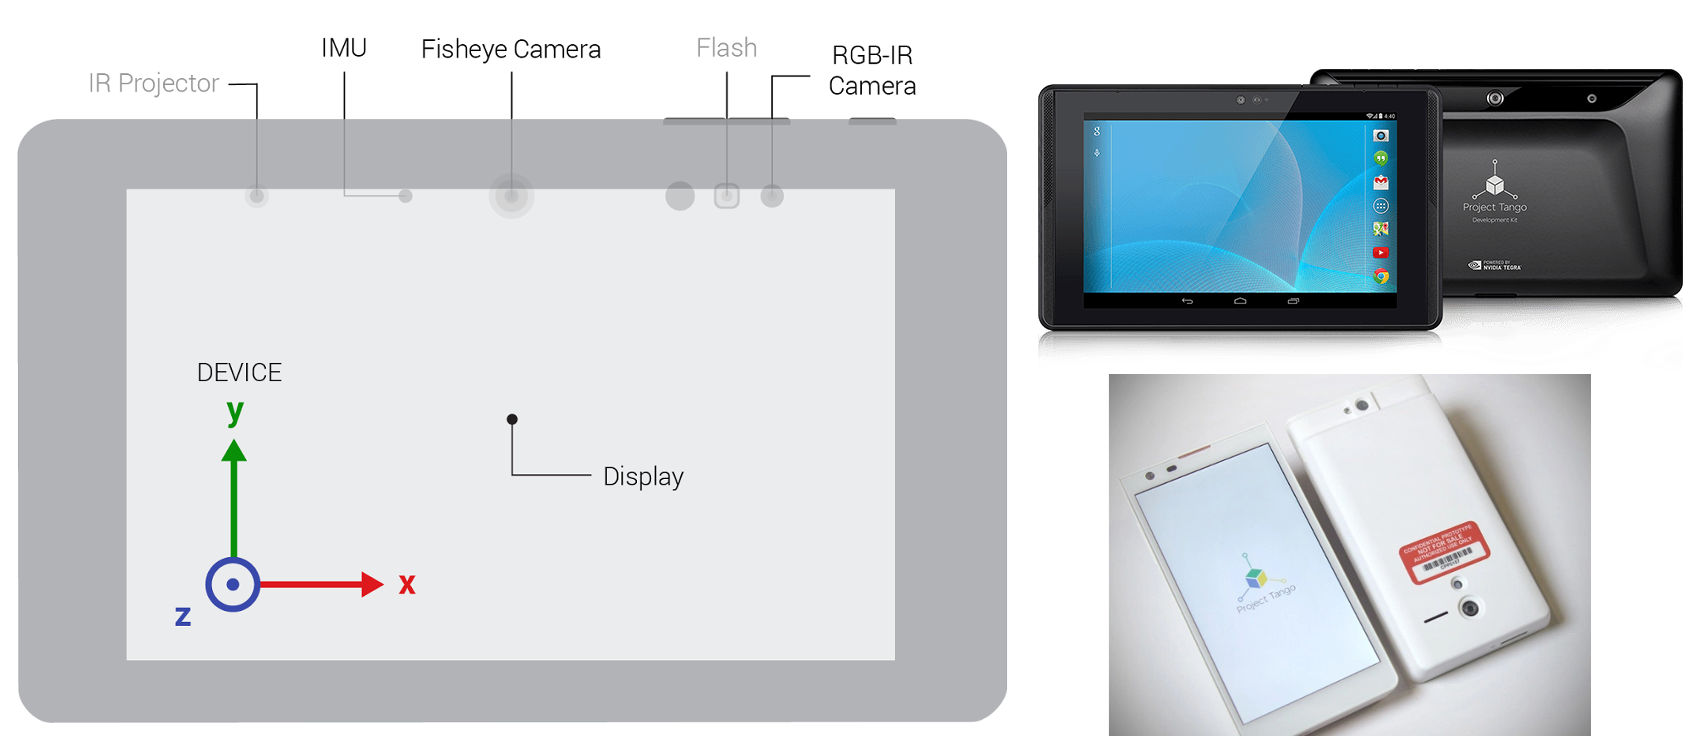
\includegraphics[width=1.0\textwidth]{content/images/theory/tango-device.png} 
  \caption{Links: schematischer Aufbau der Google Project Tango Hardware. Rechts: Das aktuelle Entwickler Gerät im Tablet Format (oben) und das alte Entwickler Gerät im Smartphone Format (unten). Übernommen von \citet{GoogleDevelopers:online}}
  \label{fig:tango-device}
\end{figure}

\subsection{Konzepte und Schnittstellen}

Generell betrachtet ist das Project Tango eine Plattform, die Computer Vision nutzt, um dem Gerät die Möglichkeit bietet seine relative Positionierung in der umgebenen Szene live zu bestimmen. Auf den Geräten kommt Googles Android zum Einsatz, weshalb zu beachten ist, dass es sich bei der Platform nur bedingt um eine Echtzeit Umgebung handelt. Das liegt daran, dass der Linux Kernel keine Garantien für die zeitlich präzise Ausführung von Instruktionen auf Grund von Scheduling geben kann. Google weist daher darauf hin, dass das System als \enquote{soft-realtime} betrachtet werden sollte. Daher sollten Messergebnisse verschiedener Sensoren unter Berücksichtigung ihrer Aufnahme Zeitpunkte verwendet werden. \citep{GoogleDevelopersConcepts:online} \\

\subsubsection{Motion Tracking}

Um die relative Bewegung vom Start des Project Tango Systems bestimmen zu können nutzt es \enquote{visual-inertial odometry}. \citep{GoogleDevelopersConcepts:online}
Dabei handelt es sich um eine erweiterte Variante von Visual Odometry. 
Das von \citet{nister2004visual} veröffentlichte Verfahren Visual Odometry ist in der Lage aus einfachen Video Inhalten in Echtzeit die Bewegung der Kamera zu bestimmen. 
Hierzu werden zunächst übergreifende Features, zum Beispiel Punkte aus der \citet{harris1988combined} Kantenerkennung, über mehrere Bilder des Videos bestimmt, woraus mit Hilfe des 5-point Algorithmus und durch Anwendung von RANSAC eine bestmögliche Approximation der Kamera Transformation bestimmt wird. \citep{nister2004visual} \\

Project Tango lässt an dieser Stelle die internen Sensoren zur Rotation, Orientierung und Bewegung mit in die Bestimmung der Kamera Transformation einfließen, um so ein akkurates Ergebnis erzielen zu können. Über eine längere Messzeit oder eine größere Entfernung vom Ursprung kann es jedoch zu kleinen Abweichungen kommen. Außerdem existiert zum aktullen Zeitpunkt noch ein \enquote{drift} Problem, was zu großen Messfehlern führen kann. Es wird jedoch versucht diese Probleme mit dem Konzept \enquote{Area Learning}, beschrieben in Kapitel \ref{subsec:area-learning}, zu lösen. \citep{GoogleDevelopersConcepts:online}
Wie genau das Verfahren aussieht, welche Techniken zur Feature Detection oder Feature Matching genutzt wird und welche Features hierfür erkannt werden ist nicht bekannt. \citet{Klingensmith_2015_7924}, als Mitglieder Googles Advanced Technologies and Projects Abteilung ATAP, erwähnen jedoch, dass nähere Informationen über das Verfahren von \citet{kottas2013consistency} und \citet{mourikis2007multi} verfasst wurden. \\

\subsubsection{Deph Perception}

Zur Tiefenmessung ist die Project Tango Hardware mit einem kalibrierten Infrarot Laser Projektor ausgestattet. Dieser streut Infrarot Punkte mit einer Auflösung von 320 x 180 Punkten in den Raum, um dann, mit Hilfe von Aufnahmen der RGB Kamera, eine Punktewolke der Tiefeninformation zu bestimmen. Auf Grund einer ausgewogenen Konfiguration zwischen Messbereich, Messfehlern und dem Energieverbrauch, liegt der Messbereich der Sensorkombination, laut \citet{GoogleDevelopersConcepts:online}, zwischen einem halben und vier Metern. \\

Dadurch dass diese Technologie auf der Aufnahme von projiziertem Infrarot Licht basiert, ist ein Einsatz der Tiefenmessung außerhalb geschlossener Räume nicht möglich. \citep{GoogleDevelopersConcepts:online} Außerdem entstehen Messfehler durch reflektierende,  lichtabsorbierende oder zu komplex strukturierte Oberflächen, wie zum Beispiel Metalle, LCD Monitore oder Hochflor Teppiche. \\

Die zuvor erwähnten Punktewolken werden in dem eigens definierten XYZij Format von der Entwicklungsschnittstelle zurück gegeben. Dabei handelt es sich pro Punkt um die \(X\),\(Y\) und \(Z\) Koordinaten sowie der Spalte \(i \) und der Zeile \(j\). \citep{GoogleDevelopersConcepts:online} Man spricht dabei von einer organisierten Punktewolke, da durch die \(i\) und \(j\) Koordinaten die direkten Nachbarn, ausgehend von dem Aufnahmeblickwinkel, eines Punktes bestimmt werden können. Hieraus ist es möglich Tiefenbilder, die sogenannten \enquote{Depth Maps}, zu bestimmen, für die es viele verschiedene Computer Vision Verfahren zur Bestimmung von Objekten, Strukturen und Fluchtpunkten gibt. Die Ermittlung der Spalten \(i\) und Zeilen \(j\) sind jedoch laut \citet{GoogleDevelopersKnownIssues:online} noch nicht in den Schnittstellen enthalten.\\ 

\citet{GoogleDevelopersConcepts:online} weist darauf hin, dass das Generieren von Polygon basierten Rekonstruktionen noch nicht in den Schnittstellen enthalten sind. Es gibt jedoch freie Dritt-Bibliotheken und -Systeme, wie das Robot Operating System \citep{ROS} oder die Point Cloud Library \citep{pcl}, die für eine weitere Verarbeitung genutzt werden können.

\subsubsection{Area Learning} \label{subsec:area-learning}

Area Learning bezeichnet den Prozess indem Project Tango Geräte in der Lage sind durch visuelle Hinweise die umgebenen Welt kennenzulernen und auf die Position des Gerätes zu schließen. 
Es ermöglicht somit eine Unterstützung für Motion Tracking und löst das Problem das Gerät in einer bereits bekannten Umgebung zu lokalisieren, wie in Abbildung \ref{fig:area-learning} links zu erkennen.
Project Tango bietet außerdem die Möglichkeit diese visuellen Hinweise und Ihre Position im Raum in sogenannten \enquote{Area Description Files} zu speichern und wiederzuverwenden. \citep{GoogleDevelopersConcepts:online}\\

\begin{figure}[h]
  \centering
	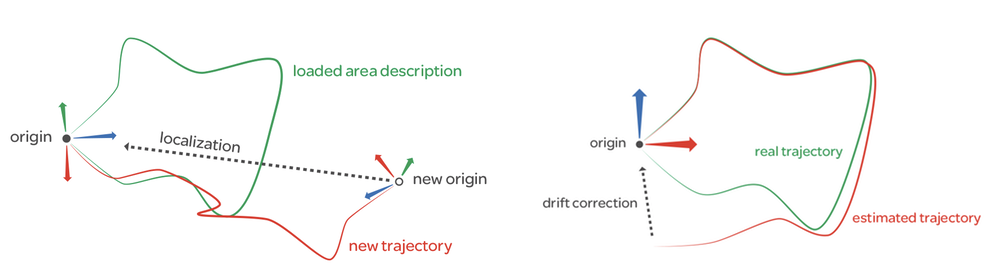
\includegraphics[width=1.0\textwidth]{content/images/theory/tango-area-learning.png} 
  \caption{Links: Lokalisierungsprozess durch Area Learning. Rechts: Korrigierung von Motion Tracking anhand gelernter Merkmale . Übernommen von \citet{GoogleDevelopers:online}}
  \label{fig:area-learning}
\end{figure}

Wie bereits erwähnt entstehen bei Motion Tracking über eine längere Strecke Messfehler. 
Während diese Strecke mit einem Project Tango Gerät abgelaufen wird, ermittelt es fortlaufend die Position und den Pfad, den der Nutzer im Raum gegangen ist. 
Erkennt es während der Strecke visuelle Merkmale aus Area Learning, wird der Pfad anhand der Positionen der Merkmale entsprechend angepasst. 
Project Tango unterscheidet hier zwischen zwei Manipulationen, \enquote{loop closures}, zur Zusammenführung des Pfads wenn ein Kreis gelaufen wurde, und \enquote{drift corrections}, um den erwähnten drift Effekt bei zu wenigen optischen Features im visual-inertial odometry. 
Die drift correction ist in Abbildung \ref{fig:area-learning} rechts zu erkennen. \citep{GoogleDevelopersConcepts:online} \\

Auch bei diesem Prozess werden die genauen Details nicht näher erläutert und es ist nicht bekannt wie die area desciptions definiert sind oder was sie enthalten. \citep{GoogleDevelopersConcepts:online} weist jedoch darauf hin, dass auch wenn die Area Desciptions Files keine direkten Bilder enthalten, es möglich sei, Rückschlüsse auf die gelernte Umgebung ziehen zu können. \\

\subsection{Einordnung zu Augmented Reality} \label{sec:classification_project_tango}

Da sowohl die Grundlagen aus dem Bereich Augmented Reality und die technische Basis von Project Tango bekannt ist, kann die Project Tango Hardware bezüglich Augmented Reality näher eingeordnet werden. Bei der Hardware handelt es sich um ein hand-held Gerät, welches mit einer video see-through Display Technologie Augmented Reality Anwendungen ermöglicht. Hierfür kann wahlweise die normale RGB Kamera oder die Graustufen Fish-Eye Kamera verwendet werden. Denn für beide Kameras können die intrinsischen Kameraparameter ausgelesen werden, wodurch die Eigenschaften realen Kamera durch die virtuelle Kamera übernommen werden können. Das führt zu einer parallax freien Überblendung und zu einer guten Tiefenwahrnehmung. \\

Als Tracking Technologie wird hier eine hybride optische Variante angewendet, die Visual Odometry mit der Fish-Eye Kamera wird durch interne Sensoren für die Rotation, Orientierung und Bewegung kombiniert. Außerdem kann das Verfahren gegebenenfalls durch Googles Area Learning Mechanismen angereichert werden, um Messfehler entgegenzuwirken. \\

Die Eingabe erfolgt durch den Touchscreen des Tablets. Eine Interaktion mit Hilfe von optischer Gestenerkennung oder anhand der Tiefeninformationen ist zudem auch möglich. \\







% Optimierung von AR
\chapter{Verfahren zur echtzeit Optimierung von Augmented Reality durch Tiefeninformationen}

\section{Verdeckung durch Depth Maps}

\section{Echtzeit Polygon Rekonstruktion} \label{sec:polygon_reconstruction}

Die Idee der Verdeckung mit Hilfe des Z-Buffers lässt sich nicht nur mit Depth Maps realisieren. Auch Primitiven oder allgemein Polygone könnten mit Hilfe eines entsprechenden Fragment Shaders, als Repräsentation der Umgebung, andere virtuelle Objekte Transparent überlagern, um die Illusion der Überdeckung von realen Objekten zu ermöglichen. Somit ließe sich das Problem der Optimierung von Augmented Reality mit Hilfe von Tiefeninformation auf das Echtzeit Rekonstruktions Problem zurückführen. \\

Die 3D Rekonstruktion ist bereits ein etabliert Forschungsgebiet in der Computer Grafik und gewinnt, auf Grund von kostengünstigen Consumer Tiefensensoren, wie die Microsoft Kinect, Asus Xtion oder Structure \citep{Struc48:online}, zunehmend an Bedeutung. Dabei wird sich immer mehr auf die Echtzeit Rekonstruktion konzentriert, da diese Geräte in der Lage sind, Tiefeninformationen, zwar mit leichten Messfehlern aber in Echtzeit, zu liefern. \citet{niessner2013real} erwähnen an dieser Stelle zudem den möglichen Einsatz für Augmented Reality:

\begin{quote}
\enquote{The ability to obtain reconstructions
in real-time opens up various interactive applications including:
augmented reality (AR) where real-world geometry can be fused
with 3D graphics and rendered live to the user; ...} \citep{niessner2013real}
\end{quote}

Die Herausforderung in der Echtzeit Rekonstruktion liegt dabei in der möglichst performanten Fusion von mehreren überlagernden Depth Maps. Hieraus soll eine möglichst detailierte Repräsentation der echten Umgebung generiert werden, welche sich im Idealfall stetig verbessert. Diese Problemstellung unterscheidet sich von herkömmlichen Rekonstruktionsverfahren wie die von \citet{hoppe1992surface} und der Poission Rekonstruktion von \citet{kazhdan2006poisson}. Aktuelle Verfahren nutzen dafür verschiedenste optimierte Datenstrukturen, welche zudem durch den Einsatz von entsprechenden GPU Implementierungen beschleunigt werden können. Dennoch spielt die Gegenüberstellung von Detailgrad, der Skalierung und Geschwindigkeit stets eine große Rolle. \citet{niessner2013real} \\

Bekannte Verfahren wie KinectFusion \citep{newcombe2011kinectfusion}, ein SLAM Verfahren von \citet{bylow2013real} oder DynamicFusion \citep{newcombe2015dynamicfusion} nutzen Truncated Signed Distance Function, kurz TSDF, zur Speicherung und Migration der Oberflächeninformation mehrerer Depth Maps. Das Verfahren von \citet{niessner2013real} erweitert diesen Ansatz mit einem effizienten Spartial Hashing Verfahren, um die Zugriffszeiten und Speicherverbrauch zu minimieren. Darüber hinaus nimmt das Verfahren Chisel von \citep{Klingensmith_2015_7924} diese Vorzüge auf und kombiniert TSDF mit  \enquote{visual-inertial odometry}, der Trackingtechnologie von Project Tango. In den folgenden Absätzen werden die Mechanismen hinter TSDF, dem räumlichen Hashing näher Erläutert. Hiernach soll auch noch auf das Rendering der TSDF Oberfläche durch Marching Cubes und auf die weiteren Optimierungen von Chisel eingegangen werden. \\


\subsection{Truncated Signed Distance Function}

Bei der von \citet{curless1996volumetric} vorgestellten räumlichen Repräsentation von Oberflächen, Truncated Signed Distance Function (TSDF), wird der Raum in Voxel einer gewünschten Auflösung unterteilt. Anders als Occupancy Maps, in denen die Voxel als sichtbar oder unsichtbar markiert werden, werden bei TSDF in den Voxeln die jeweiligen Entfernungen zur nächsten Oberfläche angegeben. Wichtig dabei ist das Vorzeichen, welches angibt, ob sich ein Voxel innerhalb oder außerhalb eines Objektes befindet.  \citep{curless1996volumetric} \\

Gefüllt wird die Repräsentation durch die Depth Maps und der entsprechenden Kameraposition, die im Fall von Project Tango bereits gegeben ist. So wird für jede Tiefeninformation ein Strahl ausgehend von der Kameraposition generiert, der die durchschnittenen Voxel aktualisiert. Der Stahl ist dabei von der Länge begrenzt, um die zu aktualisierenden Voxel zu minimieren und zudem keine Oberflächen zu aktualisieren, die sich weiter hinter der gefundenen Oberfläche befindet. Dieses Vorgehen ist in Abbildung \ref{fig:tsdf} c) zu erkennen. \citep{Compu66:online} \\

\begin{figure}
  \centering
	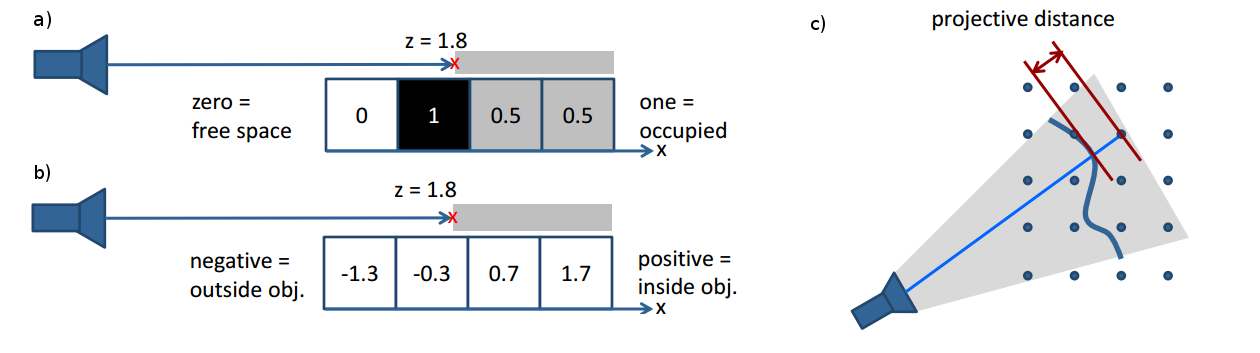
\includegraphics[width=1.0\textwidth]{content/images/methods/tsdf.png} 
  \caption{a) Beispielhafte Voxel Füllung von Occupancy Maps; b) Beispielhafte Voxel Füllung durch TSDF; c) Exemplarische 2D Darstellung der Oberfläche mit entsprechenden Strahlensatz für die TSDF. Übernommen von \citet{Compu66:online}}
  \label{fig:tsdf}
\end{figure}

Der Vorteil dieser Repräsentation liegt darin, dass die konkreten Oberflächeninformationen, anders als bei der Diskretisierung von Occupancy Maps, nicht verloren gehen. Das heißt, dass trotz einer gröberen Voxel Struktur stets der Nulldurchgang rekonstruiert werden kann. Neben der Entfernung zur nächsten Oberfläche wird zusätzlich noch ein Gewichtungswert in jedem Voxel gespeichert. Das ermöglicht es leichtes Rauschen durch einfache Mittelung zu unterdrücken und die Oberfläche optimiert sich somit bei jeder Aktualisierung der Voxel. \citep{Compu66:online}\\

\subsection{Spartial Hashing}

Das Problem der Echtzeit Rekonstruktion ist wie bereits angesprochen die Aushandlung von Detailgrad, Skalierung der zu rekonstruierenden Szene und Performance der Rekonstruktion. Auch die TSDF Repräsentation ist sehr speicherintensiv und benötigt für die zu scannende Szene reservierten Speicher, der auf mobilen Endgeräten nur begrenzt verfügbar ist. Daher muss auch für größere Rekonstruktionen oder Rekonstruktionen unbekannter Größe ein dynamischer Ansatz gefunden werden. \citet{Klingensmith_2015_7924} erwähnt dazu, dass einige Verfahren OctTrees einsetzen, die zwar äußerst dynamisch sind, jedoch einen deutlichen Nachteil hinsichtlich der Zugriffszeiten auf die Voxel bringen. \\

\begin{figure}
  \centering
	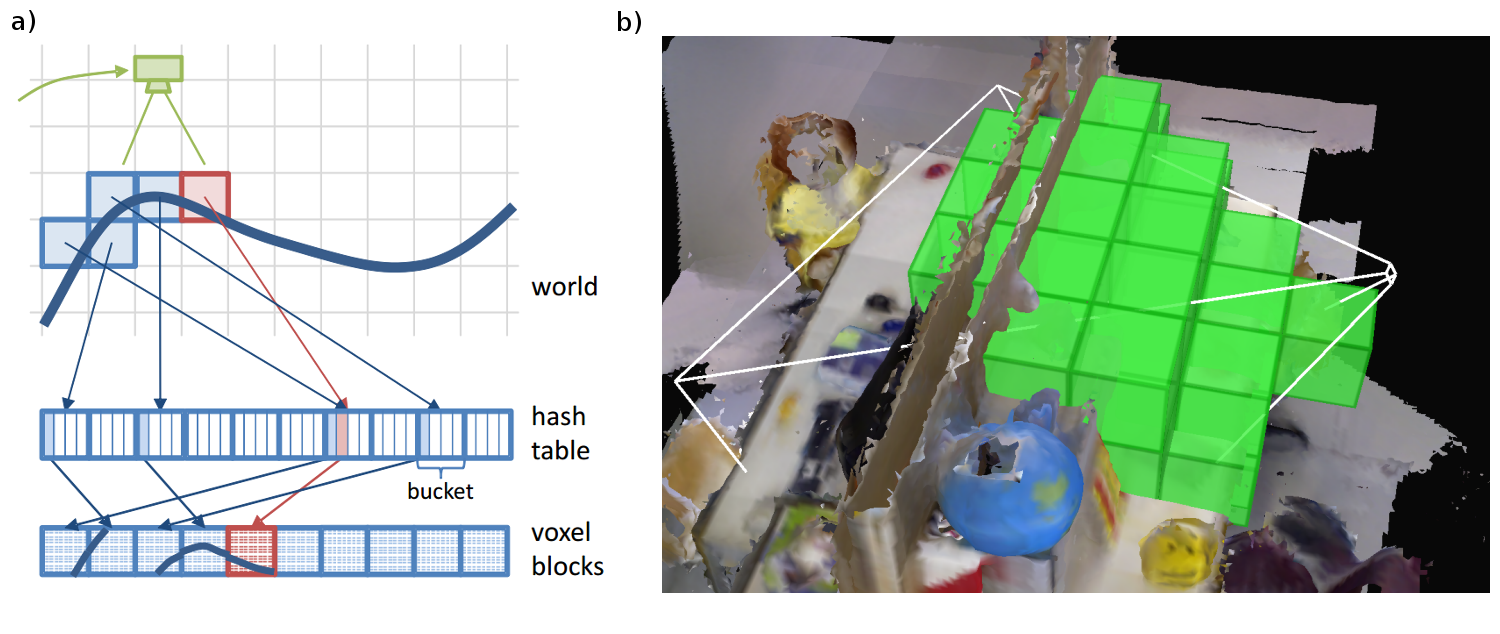
\includegraphics[width=1.0\textwidth]{content/images/methods/hashing.png} 
  \caption{a) Voxel Hashing Datenstruktur. Übernommen von \citet{niessner2013real} b) Darstellung der relevanten Voxel Chunks für die Aktualisierung. Übernommen von \citet{Klingensmith_2015_7924}}
  \label{fig:hashing}
\end{figure}

\citet{niessner2013real} führen daher eine zwei-Ebenen Baumstruktur ein, die auf der zweiten Ebene als Menge von Voxel räumlich zusammenfassen. Diese werden hier Chunks genannt. Auf der ersten Ebene können diese Chunks in einer Hash Tabelle räumlich mit einer Hashfunktion identifiziert werden. Das ermöglicht somit einen nahezu direkten Zugriff auf räumliche Voxel und ermöglicht es zudem Chunks dynamisch allokieren. Als Hash der Chunkposition \(x\), \(y\) und \(z\) wird die folgende Hashfunktion aus Gleichung \ref{eq:spatial_hash} verwendet. Bei den Variablen \(p_1\), \(p_2\) und \(p_3\) handelt es sich um willkürlich hohe Primzahlen und \(n\) entspricht der Größe der Hash Tabelle.

\begin{equation}\label{eq:spatial_hash}
H(x,y,z) = (x * p_1 \oplus y * p_2 \oplus z * p_3) \mod n
\end{equation}

\subsection{Marching Cubes}

Die meisten Echtzeit Rekonstruktionen durch TSDF wie KinectFusion sind GPU Umsetzungen, die daher die Möglichkeit besitzen ein hardwarebeschleunigtes Rendering durch Raycasting durchzuführen. Das Verfahren Chisel von \citet{Klingensmith_2015_7924} nutzt hingegen einen indirekten Weg zum Rendering durch die Marching Cubes Triangulation. \\

\begin{figure}
  \centering
	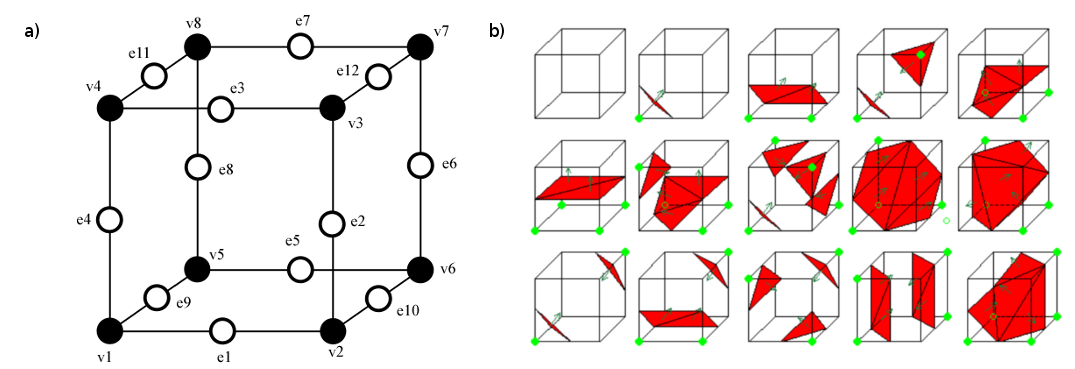
\includegraphics[width=1.0\textwidth]{content/images/methods/marchingcubes.png} 
  \caption{a) Marching Cubes Voxel Repräsentation mit den Ecken und den Kantenschnittpunkten b) Die 15 möglichen 3D Polygon Varianten. Übernommen von \citet{MarchingCubes:online}}
  \label{fig:marchingcubes}
\end{figure}

Marching Cubes nach \citet{lorensen1987marching} ist ein Algorithmus um aus einer als Voxel repräsentierten Isofläche Polygone zu bestimmen, die diese Fläche möglichst nah repräsentieren. Hierzu werden zu jedem Voxel die Ecken \(v1\) bis \(v8\) untersucht, ob sie innerhalb oder außerhalb eines Objektes liegen. Zusätzlich werden zu jeder Kante auf dem Voxel, wenn ein Schnitt der Isofläche existiert, die Schnittpunkte \(e1\) bis \(e12\) durch Diese bestimmt. Abbildung \ref{fig:marchingcubes} a) zeigt die Ecken und Kantenschnittpunkte eines Voxels. \\

Je nach binärer Gewichtung der Ecken können hiernach aus einem Katalog von 256 Varianten die Polygone nachgeschlagen werden. Inhalt des Katalogs sind die Indizes der Kantenschnittpunkte, aus denen Polygone generiert werden können. Alle diese 256 Varianten können auf 15 verschiedene Fälle zurückgeführt werden, die sich nur in Rotation oder Symmetrie unterscheiden. Die 15 Varianten sind in Abbildung \ref{fig:marchingcubes} b) zu finden. \citep{MarchingCubes:online} \\

\subsection{Chisel mit Space Carving}

Das Bereits erwähnte Verfahren Chisel von \citet{Klingensmith_2015_7924} verwendet alle zuvor erwähnten Techniken der TSDF, spartial Hashing und der Marching Cubes Überführung. Sie sprechen dabei von einem \enquote{dynamic spatial-hashed truncated distance field}. Das für den mobilen Einsatz optimierte Verfahren ist in der Lage eine Echtzeitrekonstruktion von Räumen von bis zu \(300 m^2\) mit einem Detailgrad von zwei bis drei Zentimetern zu erstellen. Zudem können neben Tiefeninformationen auch gefärbte Pointclouds verarbeitet werden, wodurch ein gefärbtes Mesh generiert werden kann. \citep{Klingensmith_2015_7924}\\

\begin{lstlisting}[mathescape,caption=Chisel TSDF Algorithmus, label=lst:chisel]
Eingabe: Pointcloud $C$, Kameratransformation $P_{cam}$, 
         Strahlenbegrenzung $t$

für jeden Tiefenwert $\vec{p}$ aus $C$
    bestimme die Oberflächenposition $\vec{z}$ aus $\vec{p}$ und $P_{cam}$
    bestimme einen Strahl $\vec{r}$ aus $\vec{z}$ und $P_{cam}$
    bestimme den Begrenzungsbereich $t_{vor}$, $t_{nach}$ mit $t$ um $\vec{z}$ auf $\vec{r}$
    # space carving
    für jeden Voxel $v$ zwischen Kamera und $t_{vor}$
        wenn die Distanz im Voxel negativ ist
            setze Voxel zurück
    # normale TSDF Bestimmung
    für jeden Voxel $v$ zwischen $t_{vor}$ und $t_{nach}$
        bestimme die Voxeldistanz zu $z$
        setze das Gewicht w des Voxels $v$
\end{lstlisting}

Zusätzlich erweitern sie den TSDF Algorithmus um die \enquote{space carving} Funktionalität. Sie betrachten dabei den Strahl von der Kamera zur Oberfläche als eine Art Constraint, in dem alle durchstoßenden Voxel bis zur Oberfläche eine negativen Wert beinhalten müssen. Ist das nicht der Fall, so wird ein Voxel außerhalb der inneren Begrenzung auf den leeren Ursprungswert gesetzt. Im Pseudocode aus Listing \ref{lst:chisel} wird das Verhalten näher erläutert. Diese Verbesserung führt dazu, dass die Rekonstruktion bei stark rauschenden Tiefeninformationen, besonders an Objektkanten, deutlich verbessert wird. Außerdem ist das Verfahren hiermit in der Lage dynamische Änderungen in der Umgebung zu detektieren und neue Oberflächen entsprechend zu aktualisieren. So beeinflussen, zum Beispiel, sich im Bild bewegen Personen nur kurz die TSDF. \citep{Klingensmith_2015_7924}\\

Neben space carving wurden zudem eine variable Strahlenbegrenzungen und Gewichtungen der Voxel abhänig von der jeweils aufgenommenen Tiefe implementiert. Diese Funktion berücksichtigt die Verteilung von Messungenauigkeiten des Sensors, die bei größerer Entfernung der Oberfläche zum Tiefensonsor zunehmen können. \citep{Klingensmith_2015_7924}

\section{Planare Rekonstruktion}

Wie bereits in Absatz \ref{sec:polygon_reconstruction} beschrieben, lässt sich das Problem der Optimierung von Augmented Reality mit Hilfe von Tiefeninformationen auf eine Echtzeit Rekonstruktion zurückführen. Im Gegensatz zur Rekonstruktion komplexer Oberflächen, mit dem vorgestellten TSDF Verfahren, soll hier eine Idee näher erläutert werden, die eine Rekonstruktion allein auf planaren Primitiven ermöglicht. \citet{yang2010plane} erwähnt hierzu, dass Ebenen in fast allen künstlichen Umgebungen zu finden sind und auf Grund ihrer vorteilhaften geometrischen Eingenschaften in verschiedensten Computer Vision Verfahren verwendet werden. Daher gibt es viele Forschungsarbeiten, Methoden und Algorithmen um aus verschiedensten Informationsquellen ein Ebenenmodell zu extrahieren.\\

Wie in dem \enquote{Simultaneous Localization and Mapping} (SLAM) Verfahren von \citet{trevor2012planar} wird hier zunächst eine Ebene in der Pointcloud mit Hilfe des RANSAC Algorithmus gesucht. RANSAC bietet gegenüber anderen Algorithmen zur Ebenen Detektion den Vorteil, ein Modell auch bei vielen Ausreißern performant zu ermitteln. Agglomeratives Clustering und Region Growing wie von \citet{feng2014fast} beschreiben, eignet sich auf Grund des Ausgabeformats aus Project Tango nicht, da es keine organisierte Point Cloud ausgibt. \\

Die Repräsentation der Ebene \(P\) wird, angelehnt an das Vorgehen von \citet{trevor2012planar}, wie in Gleichung \ref{eq:plane} festgehalten. Dabei handelt es sich um den Normalenvektor \(\vec{n}\) und der Distanz zum Ursprung \(d\) der Hesse Normalform einer Ebene, sowie der Punkte der konvexen Hülle \(H\). Um die konvexe Hülle der Ebene zu bestimmen, wird der Graham Scan Algorithmus verwendet. Wie auch von \citet{trevor2012planar} beschreiben wird die konvexe in der Repräsentation festgehalten, um eine sukzessive Verbesserung einer Ebene nach mehreren Messdurchläufen zu ermöglichen. So werden die Punkte der konvexen Hülle pro Messvorgang kombiniert, damit die Ebenenausbreitung auch außerhalb des Sichtfeldes beibehalten werden kann.

\begin{equation} \label{eq:plane}
P=\left[\vec{n}, d, H\right] \qquad H=\vec{h_1}, \vec{h_2}, \ldots  \vec{h_n}
\end{equation}

Um wiederum aus dieser Repräsentation eine Triangulation zu erhalten, wird hier die zweidimensionale Sweep-Line Delaunay Triangulation durchgeführt. Die Schritte aus dem Algorithmus \ref{lst:planeReconstruction} werden in den folgenden Kapiteln näher beschreiben.

\begin{lstlisting}[mathescape,caption=Algorthmus der planaren Echtzeit Rekonstruktion, label=lst:planeReconstruction]

Eingabe: Octtree $O$
Ausgabe: Polygonpunkte $T_{Gesamt}$

für jedes Cluster $C$ aus $O$
    bestimme Ebene [$\vec{n}$, $d$, $P$] mit RANSAC aus $C_{Punkte}$
    wenn keine Ebene mit genügend $P$ in $C_{Punkte}$ gefunden wurde
    		nächstes Cluster (continue)
    wenn Ebene mit [$\vec{n}$, $d$, $H_{alt}$] in $C_{Ebenen}$ existiert	
        füge die konvexe Hülle $H_{alt}$ zu $P$ hinzu	
    bestimme die konvexe Hülle $H_{neu}$
    bestimme die Tringulation $T_{Ebene}$ aus $H_{neu}$
    $T_{Gesamt}$ += $T_{Ebene}$
    $C_{Ebenen}$ += [$\vec{n}$, $d$, $H_{neu}$]
    $C_{Punkte}$ - $P$
		

\end{lstlisting}

\subsection{RANSAC zur Ebenendetektion}

Der \enquote{RAndom SAmple Consensus} Algorithmus (RANSAC), vorgestellt von \citet{fischler1981random}, ist in der Lage, aus einer Menge von Daten mit vielen Ausreißern, die Parameter für ein passendes Modell zu schätzen. Anders als andere Schätzverfahren wie \enquote{Least-Median} oder \enquote{M-Schätzer}, welche aus der Statistik Literatur entnommen und entsprechend angepasst wurden, wurde RANSAC speziell für die Anwendung in der Computer Graphik entwickelt. Der Kern dieses Algorithmus ist das wiederholte Bestimmen eines Modells aus zufälligen und für das Modell ausreichenden Stichproben. Listing \ref{lst:ransac} zeigt den Verlauf des RANSAC Algorithmus. Die Anzahl der Iterationen \(N\) hängt dabei allein von dem Anteil der Ausreißer in den Messwerten ab. Daher sollte sie entsprechend gewählt werden, um die Wahrscheinlichkeit zu verringern, dass Ausreißer in den Stichproben enthalten sind. \citep{derpanis2010overview} \\

\begin{lstlisting}[mathescape,caption=Der RANSAC Algorithmus, label=lst:ransac]
Eingabe: Messwerte $P$, Modelltoleranz $e$, maximale Iterationen $N$
Ausgabe: Modell $m$, Unterstützende Messwerte $P_m$

1. Wähle zufällig so viele Stichproben aus den Messwerten $P$,
   wie nötig sind, um das Modell zu bestimmen
2. Bestimme aus den gewählten Stichproben das Modell $m$
3. Ermittle die Anzahl der Messwerte $P$, die mit einer 
   entsprechenden Toleranz $e$ das ermittelte Modell $m$ 
   unterstützen
4. Wenn prozentual genügend Messwerte aus $P$ das Modell $m$ 
   unterstützen, ermittle aus den unterstützenden Messwerten 
   $P_m$ durch lineare Regression erneut das finale Modell 
   $m$ und terminiere
5. Wiederhole die Schritte 1-4 $N$ mal
\end{lstlisting} 

Um mit dem RANSAC Algorithmus Ebenen in einer Punktewolke bestimmen zu können, werden pro Iteration drei Stichproben \(A\), \(B\) und \(C\) gewählt. Das Ebenenmodell, hier in der Hesse Normalform mit dem Normalenvektor \(\vec{n}\) und dem Abstand zum Koordinatenursprung \(d\), lässt sich dabei durch die Gleichung \ref{eq:normalform} bestimmen.

\begin{equation}\label{eq:normalform}
\vec{n} =\left|\left| \vec{AB} \times \vec{AC}\right|\right|
\qquad
\vec{D} = \vec{A} \cdot \vec{n}
\qquad
d = D_1 + D_2 + D_3
\end{equation}

Um zu ermitteln ob ein Punkt \(P\) aus einer Messreihe die gefundene Ebene \(\left[\vec{n_E}, d_E\right]\) unterstützt, wird die kürzeste Distanz \(d_P\) zwischen Punkt und Ebene wie in Gleichung \ref{eq:plane-distance} ermittelt.  Ein entsprechender Toleranzwert für die Distanz \(d_{min}\), im gezeigten RANSAC Algorithmus \(e\) genannt, wird später bei der Umsetzung abhängig vom Rauschen des Tiefensensors gewählt. 

\begin{equation} \label{eq:plane-distance}
d_P = n_1*P_1+n_2*P_2+n_3*P_3-d_E \qquad support_{d_P} = d_P < d_{min}
\end{equation}

Um das finale Modell der Ebene zu ermitteln, und somit die Varianz des Abstands der Punkte zur Ebene zu minimieren, wird mit Hilfe der unterstützenden Punkte \(P_{support}=\left[x,y,z\right]\) eine lineare Regression durchgeführt. Diese Mittelt ein Ebenenmodell \(E=\left[a,b,c\right]\) aus den zuvor ermittelten Punkten mit Hilfe des \enquote{least squares} Schätzverfahren. Für eine Ebene versucht man die Funktion \(G(a,b,c)\) aus Gleichung \ref{eq:least-squares} zu minimieren. Hierzu muss das lineare Gleichungssystem in Gleichung \ref{eq:least-squares-solution}  gelöst werden. \citep{Regre94:online}

\begin{equation} \label{eq:least-squares}
z = ax + by + c   \qquad G(a, b, c) = \sum {\left(z_i - ax_i - by_i - c\right)}^2
\end{equation}

\begin{equation} \label{eq:least-squares-solution}
\begin{bmatrix}
\sum x_i^2 & \sum x_iy_i & \sum x_i\\ 
\sum x_iy_i  & \sum y_i^2  & \sum y_i \\ 
\sum x_i & \sum y_i  & n
\end{bmatrix}
*
\begin{bmatrix}
a\\ 
b\\ 
c
\end{bmatrix}
=
\begin{bmatrix}
\sum x_iz_i\\ 
\sum y_iz_i\\ 
\sum z_i
\end{bmatrix}
\end{equation}

\subsection{Bestimmung der Ebenenausbreitung}

Nachdem die Ebene und die korrespondierenden Punkte zur Ebene gefunden wurden, muss noch die Ausbreitung der Fläche bestimmt werden, da die Ebene in Hesse Normalform lediglich die Position \(\vec{n} * d\) und Ausrichtung \(\vec{n}\) festhält. \citet{PlanarSurfaceMapping} nutzt hierfür die konvexe Hülle der korrespondierenden Punkte und trianguliert diese. Um das performant umzusetzen, kann man sich hier die Eigenschaft der Ebene zu Nutzen machen und die dreidimensionalen Punkte durch Parallelprojektion als zweidimensionale Punkte auf die Ebene projizieren. Denn die Algorithmen für die Triangulation haben im zweidimensionalen eine deutlich besseres Laufzeitverhalten. \\

Nach der Triangulation können die Ecken der gefundenen Polygone jeweils zurück projiziert werden. Die Gleichungen \ref{eq:projection2d} und \ref{eq:projection3d} bilden die Projektion der Punkte wobei \(R_{\vec{n}to\vec{z}}\) der Rotationsmatrix zwischen dem Normalenvektor \(\vec{n}\) und der Z-Achse \(\vec{z}\) entspricht.\\

\begin{equation} \label{eq:projection2d}
p_{2d} = (p_{3d} - (\vec{n}*d)) * R_{\vec{n}to\vec{z}}
\end{equation}
\begin{equation} \label{eq:projection3d}
p_{3d} = (p_{2d} * R_{\vec{n}to\vec{z}}^{-1}) + (\vec{n}*d)
\end{equation}

\subsubsection{Convex Hull Algorithmus}

Für die Berechnung der konvexen Hülle wird der Graham Scan nach \citet{graham1972efficient} genutzt. Dieser Algorithmus besitzt eine Laufzeit von \(O(n \log n)\) und gilt als einer der populärsten Algorithmen für die Berechnung der konvexen Hülle. Andere Ansätze besitzen dabei ein ähnliches oder schlechteres Laufzeitverhalten. Gestartet wird der Algorithmus mit der Menge aller Punkte \(P\) der Ebene und mit einem Startpunkt \(P_0\), der Bestandteil der konvexen Hülle ist. Hierzu wird meist der Punkt mit dem niedrigsten \(y\) Faktor gewählt. (\(P_0=P_{min(y)}\)) Listing \ref{lst:graham-scan} zeigt den Verlauf des Algorithmus des Graham Scans. Dabei wird in Abbildung \ref{fig:convexhull} nochmals die erste Sortierung und das Unterscheidungskriterium für die Sortierung als auch für die Aussortierung der Punkte verdeutlicht. \citep{convexHull} \\

\begin{figure}
  \centering
	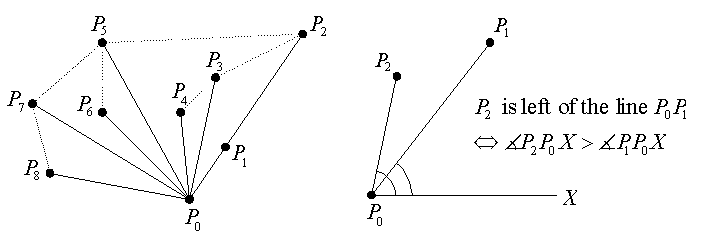
\includegraphics[width=0.9\textwidth]{content/images/methods/convexhull.png} 
  \caption{Sortierung der Punkte nach Winkel zum Startpunkt (links) mit dem Unterscheidungskriterium (rechts). Übernommen von \citet{convexHull}}
  \label{fig:convexhull}
\end{figure}

\begin{lstlisting}[mathescape,caption=Graham Scan Algorithmus, label=lst:graham-scan]
Eingabe: Menge der Punkte $P$, außen liegender Punkt $P_0$
Ausgabe: Punkte der konvexen Hülle

$i$ = 0
sortiere nach dem Winkel zu $P_0$
solange $i$ <= $|P|$
    wenn $\measuredangle P_{i-1} P_{i}$ > $\measuredangle P_{i-1} P_{i+1}$, also $P_i$ rechts von  $\vec{P_{i-1} P_{i+1}}$ liegt
        inkrementiere $i$
    ansonsten
        entferne $P_i$ aus $P$
        dekrementiere $i$
    
\end{lstlisting} 


\subsubsection{Triangulation}

Nachdem die konvexe Hülle bestimmt wurde, müssen die Punkte dieses Pfades noch trianguliert werden. Hierfür wird eine Delaunay-Triangulation mit Hilfe des Sweep-Line Algorithmus von \citet{domiter2008sweep} verwendet. Unter einer Delaunay-Triangulation versteht man zunächst einmal eine Art Constraint, der sogenannten Umkreisbedingung, die besagt, dass ein Kreis, der alle drei Punkte eines gefundenen Polygons durchzieht, keine weiteren Punkte beinhalten darf. \\

Nähere Beschreibung des Algorithmus ...

\subsection{Planare Rekonstruktion als Echtzeit Umsetzung}

\subsubsection{Clusteringverfahren}



% Umsetzung
\chapter{Umsetzung der Verfahren}

Dieses Kapitel widmet sich der Umsetzung der in der praktischen Umsetzung der beschriebenen Verfahren zur Echtzeit Planaren oder Polygon Rekonstruktion. Außerdem werden zunächst die allgemeinen technischen Problemstellungen bezüglich Project Tango beschrieben und eine Umsetzung vorgestellt, wie man mit Tiefeninformationen in Augmented Reality interagieren kann.


\section{Project Tango: Technische Grundlagen}

\section{Echtzeit Verdeckung durch Depth Maps}

\section{Echtzeit Polygon Rekonstruction}

\section{Echtzeit Planare Rekonstruction}


% Evaluation
\chapter{Evaluation}

In diesem Kapitel sollen die beschriebenen und prototypisch implementierten Verfahren zur Überlagerung gegenübergestellt werden, um anhand eines direkten Vergleichs eine objektive Aussage über die Qualität der Ergebnisse treffen zu können. Hierzu wird im ersten Teil das Vorgehen zum Testen vorgestellt, welches darauf folgend mit allen Verfahren umgesetzt wird. Hiernach werden die daraus resultierenden Ergebnisse gegenübergestellt.

\section{Statische Testszenen}

Zum Vergleich der Verfahren wurden zwei statische Szenen gewählt, in denen das Project Tango Gerät nicht bewegt wird und für alle Kandidaten den selben Inhalt bietet. Diese Wahl wurde getroffen, um eine zuverlässige und reproduzierbare Informationsquelle für das Gerät zu schaffen. Denn die Reproduktion eines bewegten und dynamischen Szenarios ist für alle zu vergleichenden Verfahren nur sehr schwer möglich. \\

Eine mögliche Idee für ein dynamisches Testszenario war es, alle sensorischen Informationen der Hardware einmal aufzunehmen und eine reproduzierbare simulierte Umgebung dieser Daten zu schaffen. Technologien wie das Robot Operating System (ROS) würden dies ermöglichen, jedoch übersteigt der Aufwand den zeitlichen Rahmen dieser Arbeit. Auch wenn die Firma Bosch eine exemplarische Implementation\footnote{Tango Output to Rosbag Files - https://goo.gl/hhnciZ} für die Aufnahme aller Daten in ROS demonstriert, sind die implementierten Verfahren zu sehr in den API Zyklen der Project Tango Schnittstelle involviert, um diese in kurzer Zeit auf eine Desktop Umgebung zu portieren.\\

Die erste gewählte Szene, welche in Abbildung \ref{fig:static-scene} links zu sehen ist, beinhaltet einen Hocker, in Form eines einfachen  Würfels, und einen Sitzball. Der Sitzball wurde gewählt, um auch runde Formen zur Tiefenaufnahme zu testen. Das Project Tango Gerät ist etwas höher in einem Stativ plaziert. Das virtuelle Objekt wird, wie in Abbildung \ref{fig:static-scene} rechts, zwischen die beiden realen Objekte plaziert, sodass es von beiden Seiten durch die realen Objekte überdeckt wird. \\

\begin{figure}[h]
  \centering
	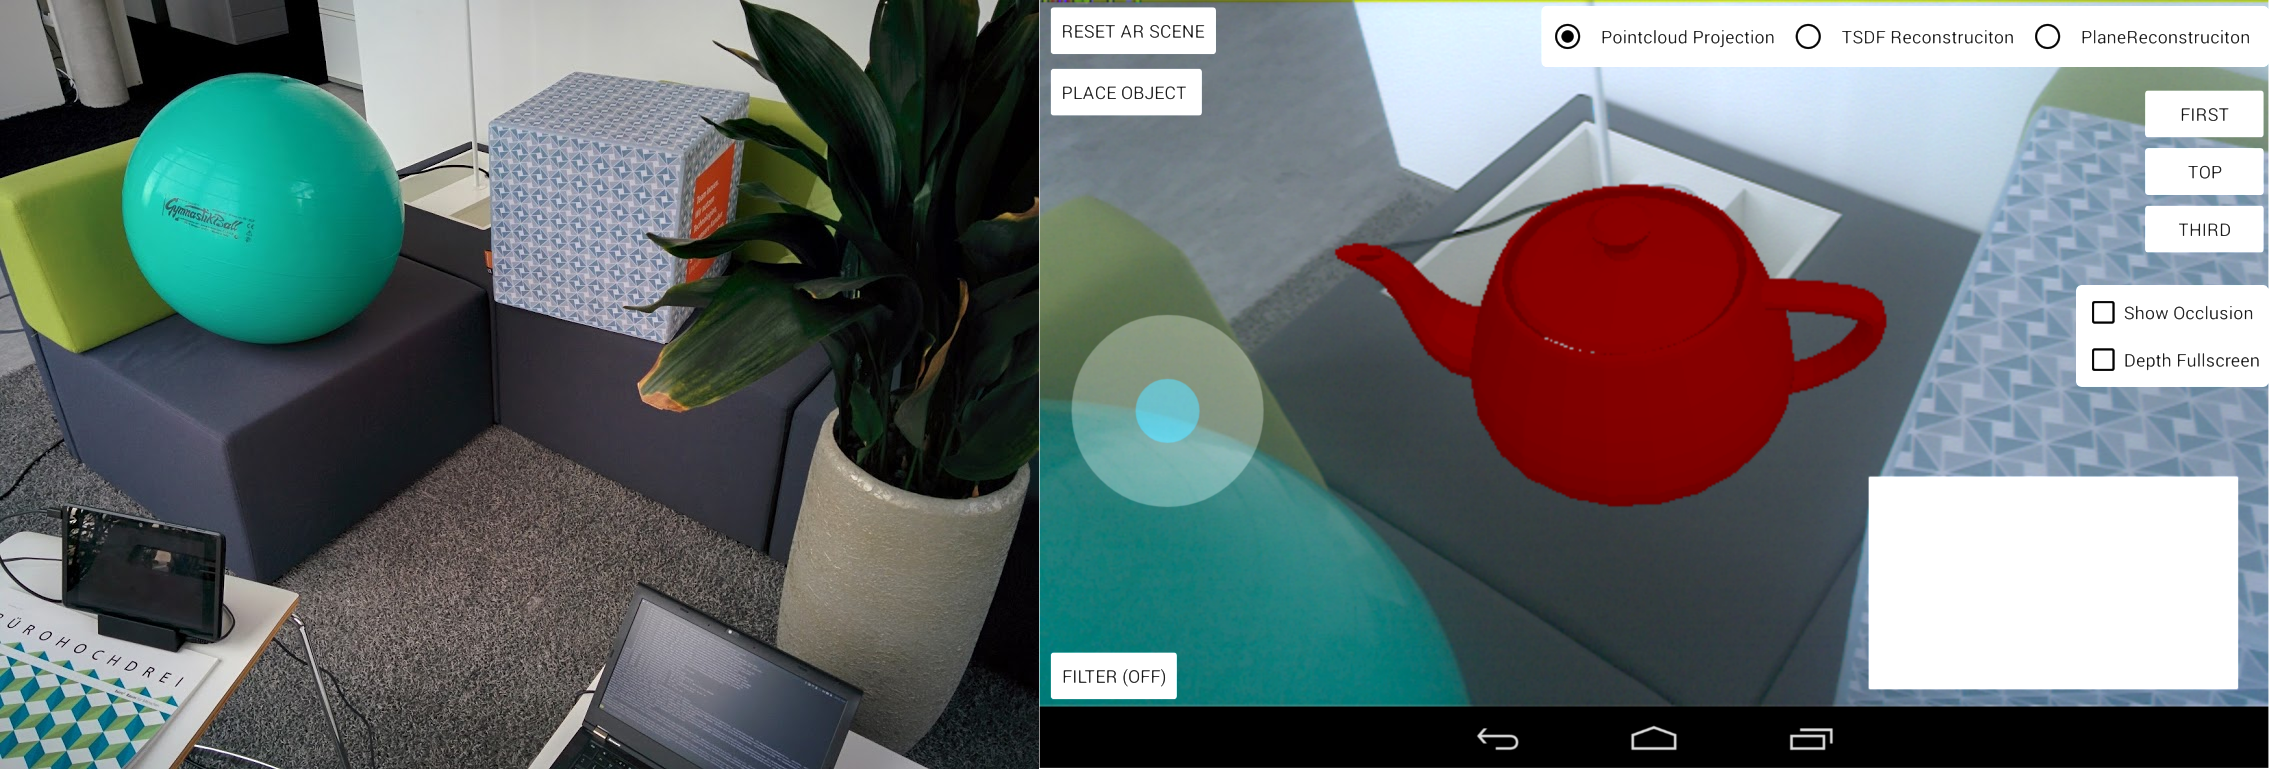
\includegraphics[width=1.0\textwidth]{content/images/evaluation/static-scene.png} 
  \caption{Links: Erste statische Szene mit einem Hocker und einem Sitzball. Rechts: Platzierung des virtuellen Objekts. }
  \label{fig:static-scene}
\end{figure}

Die zweite gewählte Szene, welche in Abbildung \ref{fig:plant-scene} links zu sehen ist, soll als Herausforderung die Überdeckung von komplexeren Strukturen testen. Sie besteht daher aus einer Pflanze, die sich, wie rechts im Bild zu sehen, vor dem virtuellen Objekt befindet. Auch hier befindet sich das Project Tango Gerät in einem Stativ.

\begin{figure}[h]
  \centering
	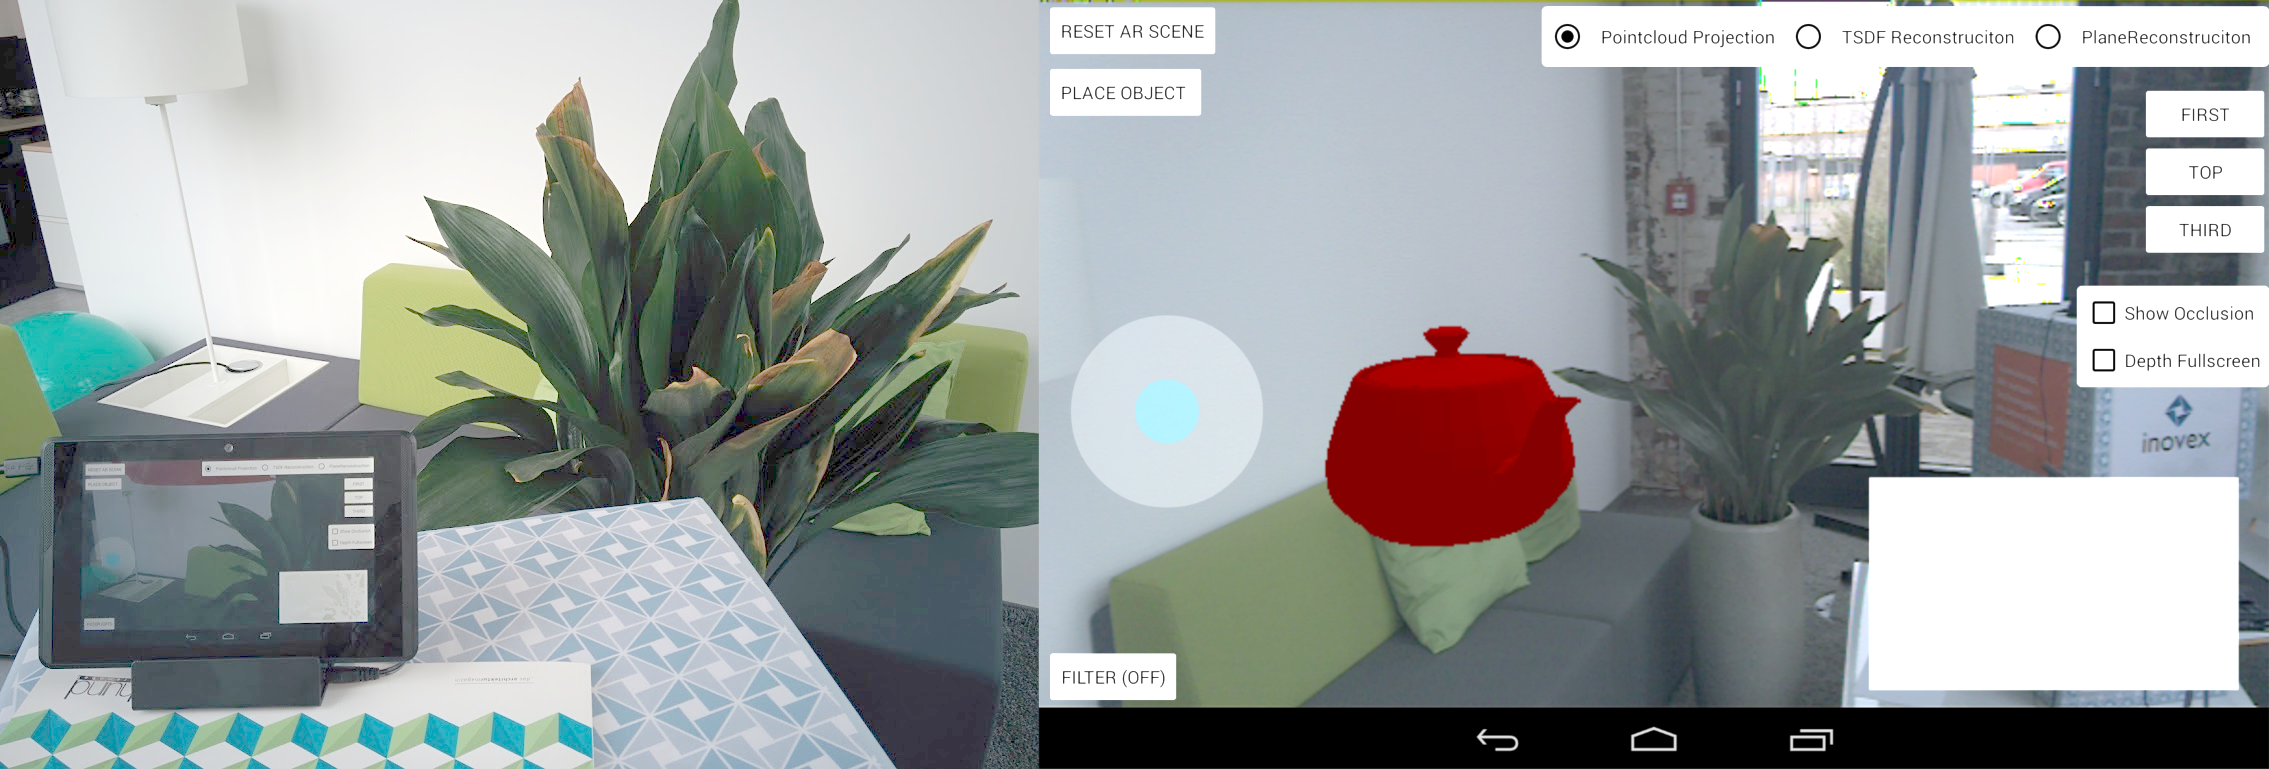
\includegraphics[width=1.0\textwidth]{content/images/evaluation/plant-scene.png} 
  \caption{Links: Zweite statische Szene mit einer Pflanze im Vordergrund. Rechts: Platzierung des virtuellen Objekts hinter der Pflanze. }
  \label{fig:plant-scene}
\end{figure}

Für beide Szenen sollen alle Kombinationen der Verfahren getestet werden. Somit ergeben sich sechs verschiedene Kombinationen, in denen die Pointcloud Projektion, die TSDF Rekonstruktion und die Ebenen Rekonstruktion jeweils mit und ohne dem Guided Filter getestet werden. Für alle Kombinationen soll ein gerendertes Bild und ein Tiefenbild mit dem virtuellen Objekt festgehalten werden. Zur Auswertung werden die jeweils gerenderten Ergebnisbilder mit einem manuell zugeschnittenem Ergebnisbild verglichen. Hierfür wird die Summe der absoluten Bilddifferenz wie in Gleichung \ref{eq:diff} bestimmt.

\begin{equation} \label{eq:diff}
d = \sum_i |p_i-q_i|
\end{equation}

\section{Durchführung der Tests}

\begin{figure}[h]
  \centering
	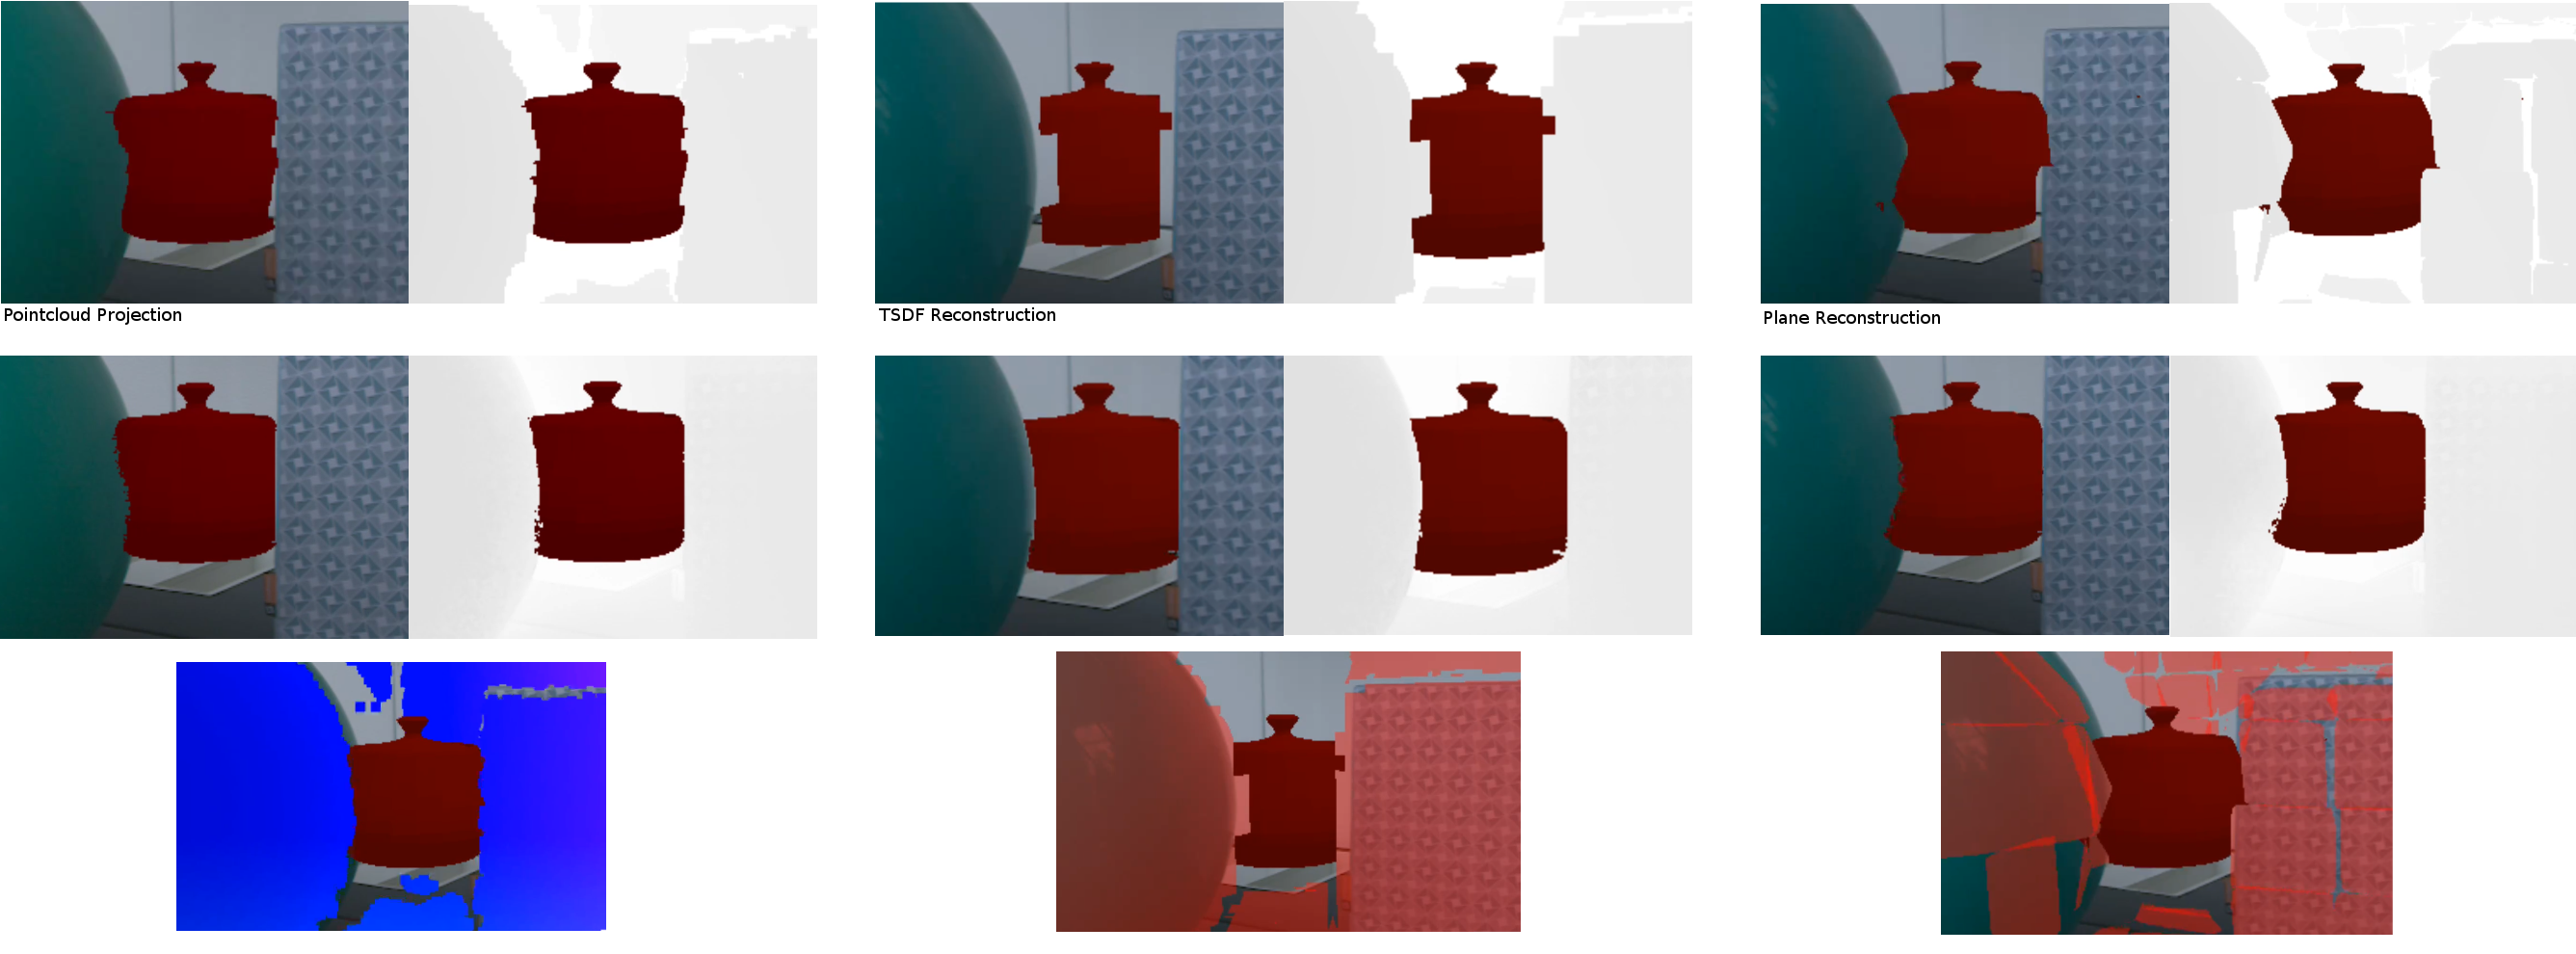
\includegraphics[width=1.0\textwidth]{content/images/evaluation/static_occlusion.png} 
  \caption{}
  \label{fig:static_occlusion}
\end{figure}

\begin{figure}[h]
  \centering
	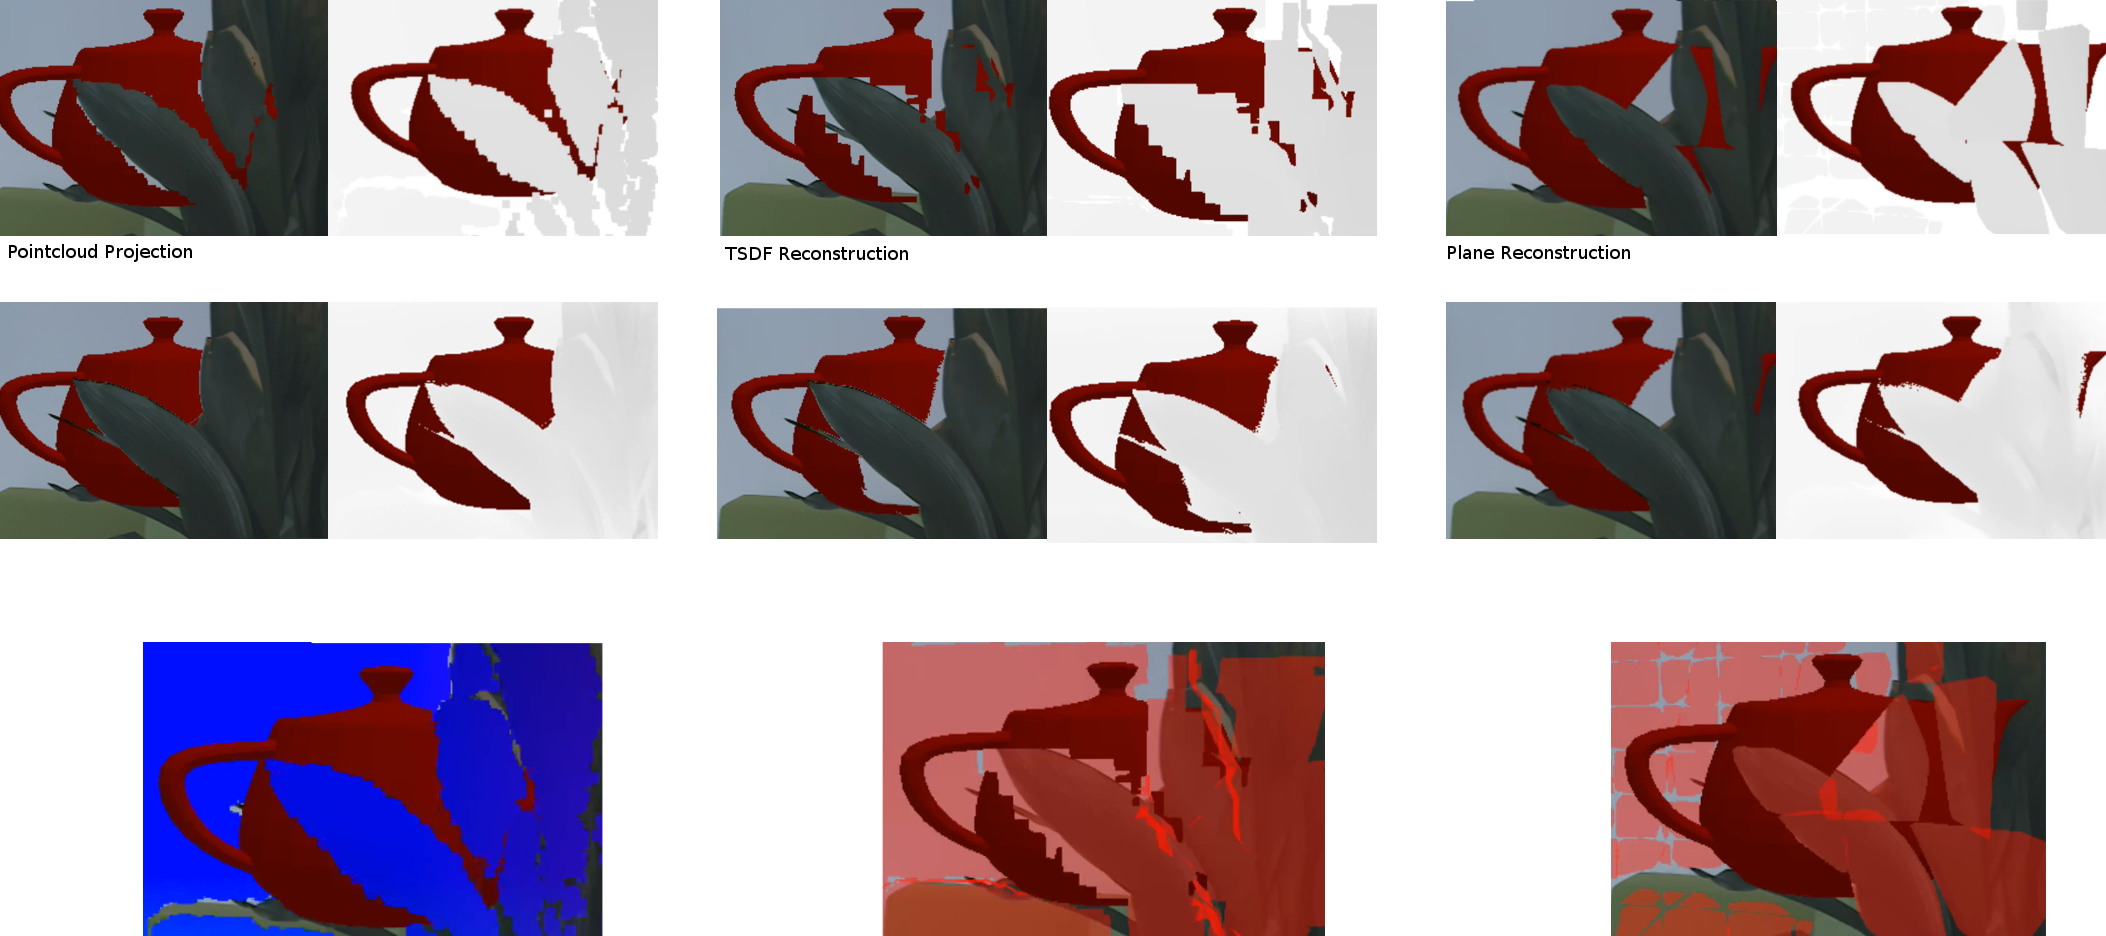
\includegraphics[width=1.0\textwidth]{content/images/evaluation/plant_occlusion.png} 
  \caption{}
  \label{fig:plant_occlusion}
\end{figure}

\section{Vergleich der Ergebnisse}

\begin{figure}[h]
  \centering
	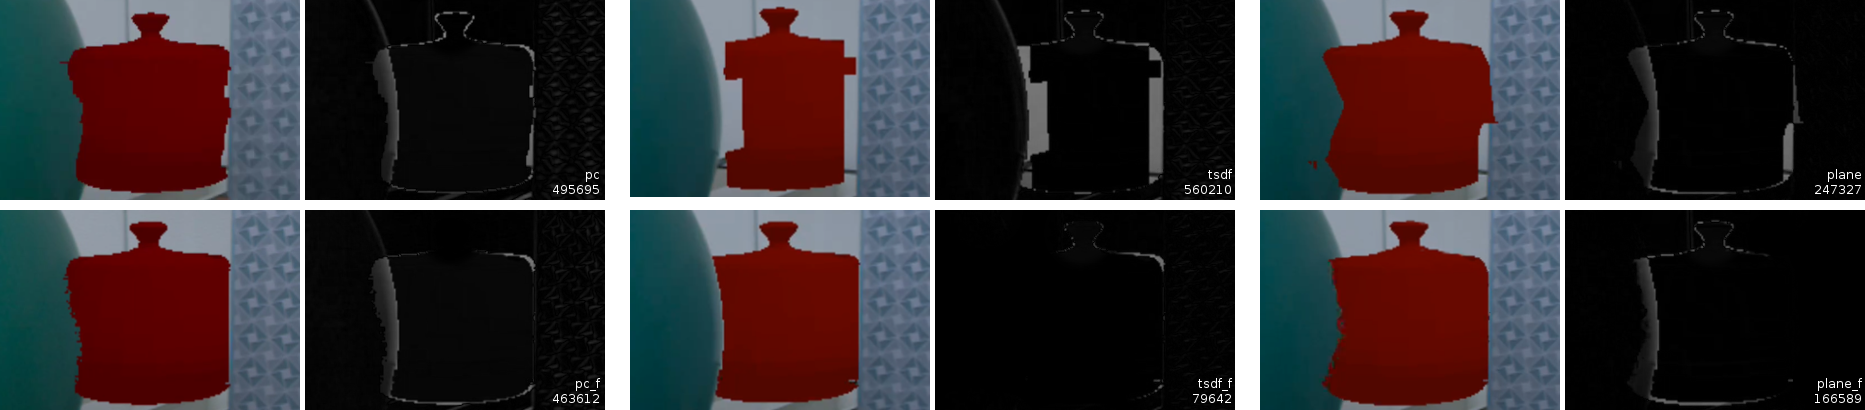
\includegraphics[width=1.0\textwidth]{content/images/evaluation/static_occlusion_results.png} 
  \caption{}
  \label{fig:static_occlusion_results}
\end{figure}

\begin{figure}[h]
  \centering
	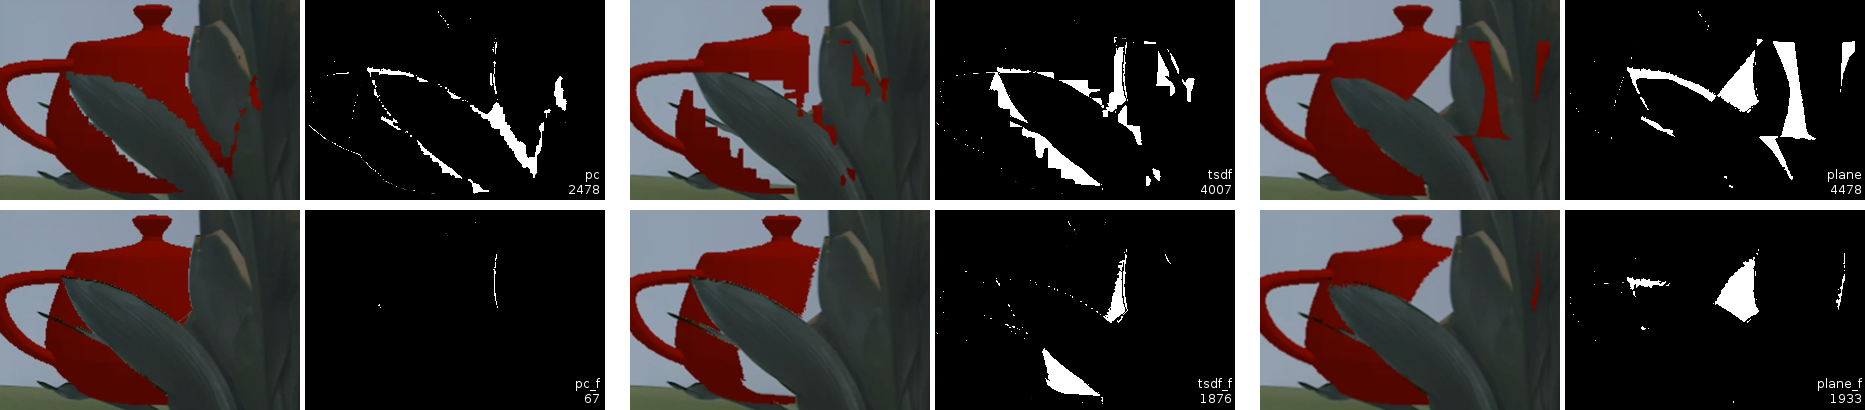
\includegraphics[width=1.0\textwidth]{content/images/evaluation/plant_occlusion_results.png} 
  \caption{}
  \label{fig:plant_occlusion_results}
\end{figure}

% Fazit
\chapter{Fazit}

* Light-Field Cameras als Kombination für AR!!


\appendix
\listoffigures
\lstlistoflistings        
%\chapter{Ergebnisaufnahmen}
\begin{sidewaysfigure}[h]
  \centering
	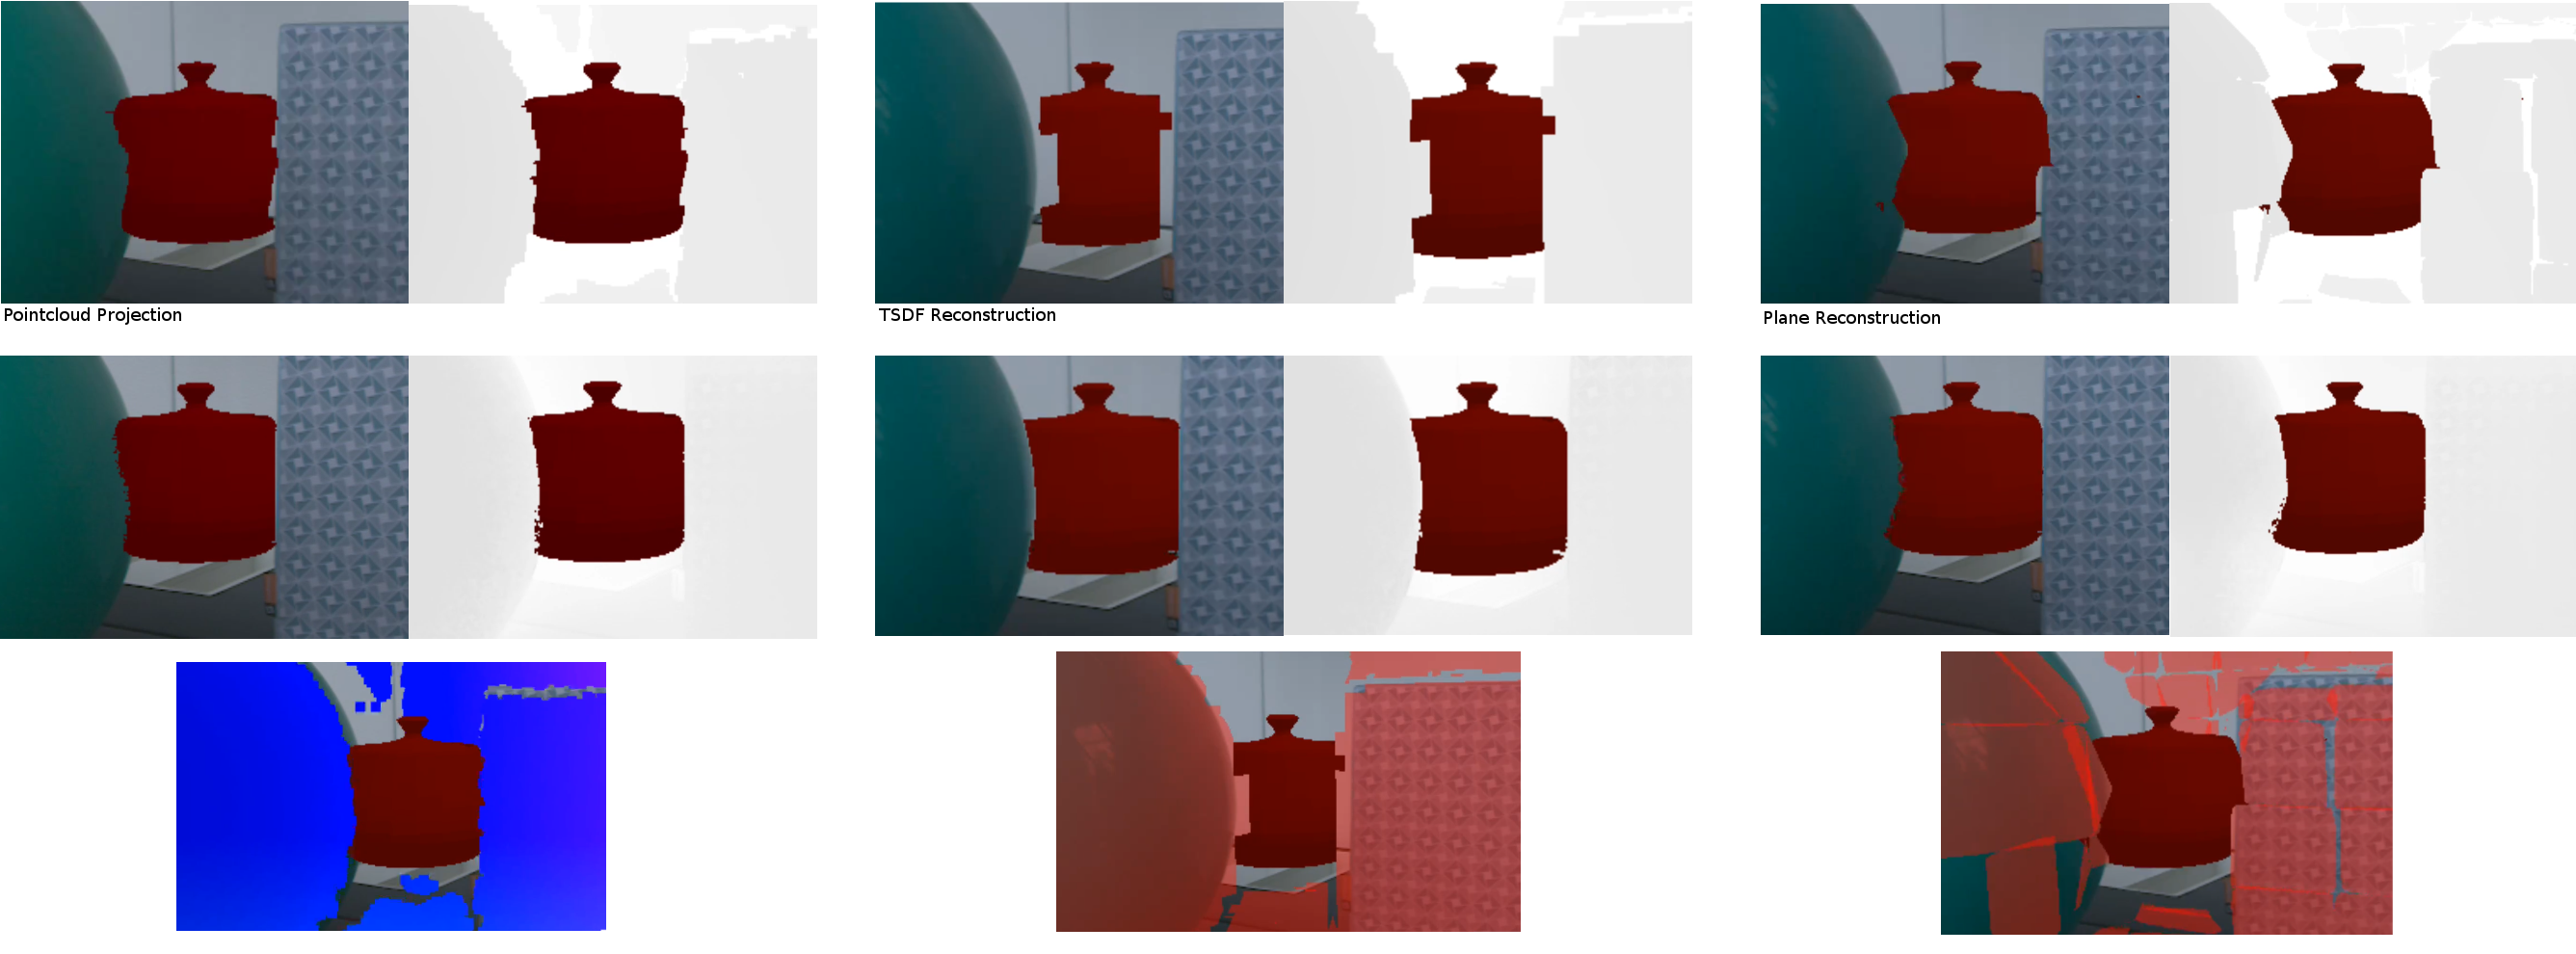
\includegraphics[width=1.0\textwidth]{content/images/evaluation/static_occlusion.png} 
  \caption{Ergebnisaufnahmen aus der ersten statischen Szene}
  \label{fig:static_occlusion}
\end{sidewaysfigure}

\begin{sidewaysfigure}[h]
  \centering
	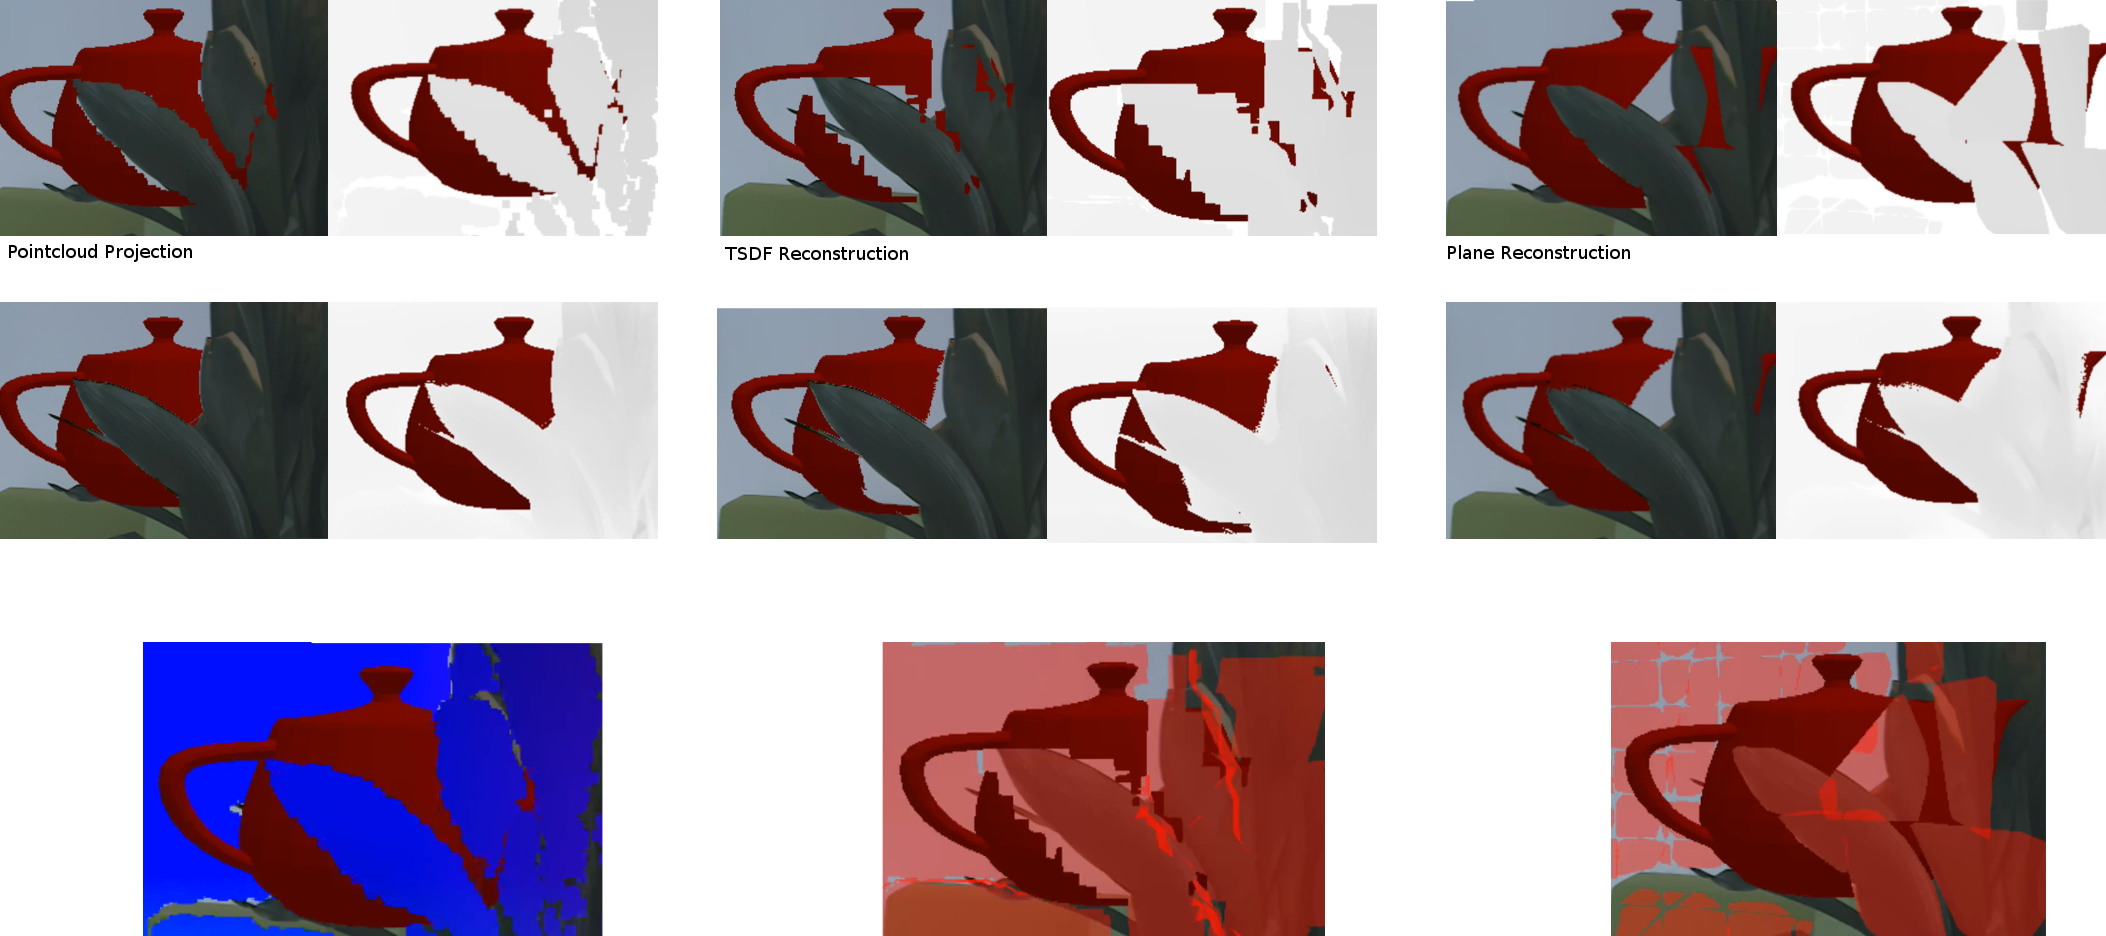
\includegraphics[width=1.0\textwidth]{content/images/evaluation/plant_occlusion.png} 
  \caption{Ergebnisaufnahmen aus der zweiten statischen Szene}
  \label{fig:plant_occlusion}
\end{sidewaysfigure}

\begin{sidewaysfigure}[h]
  \centering
	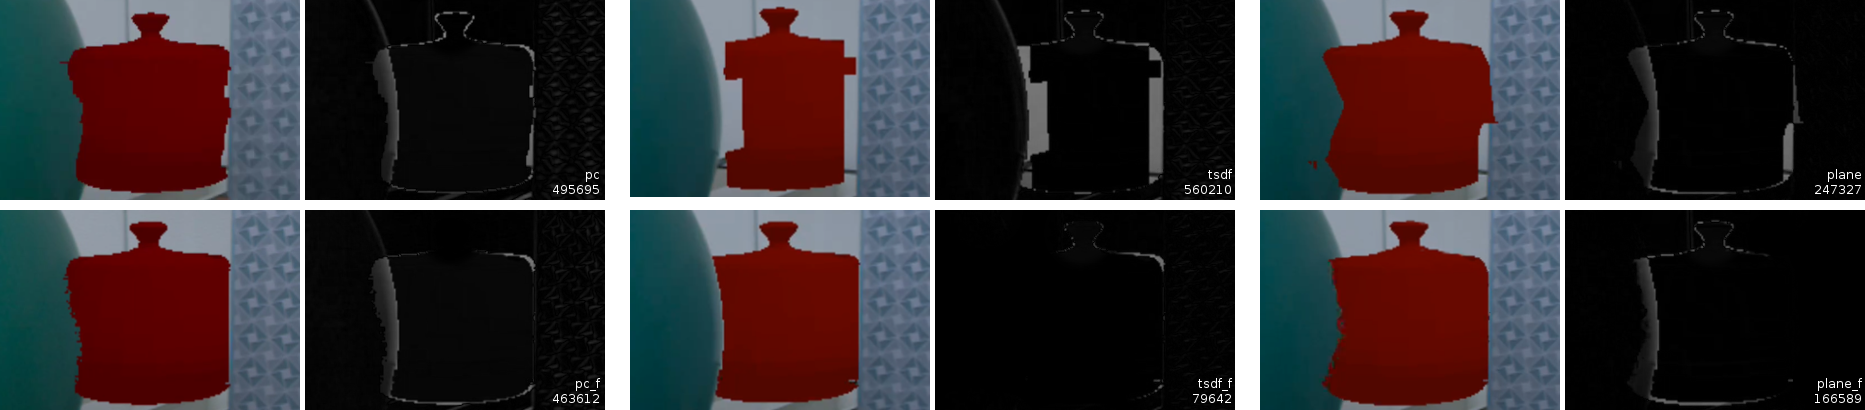
\includegraphics[width=1.0\textwidth]{content/images/evaluation/static_occlusion_results.png} 
	
\includegraphics[width=1.0\textwidth]{content/images/evaluation/spacer.png} 
	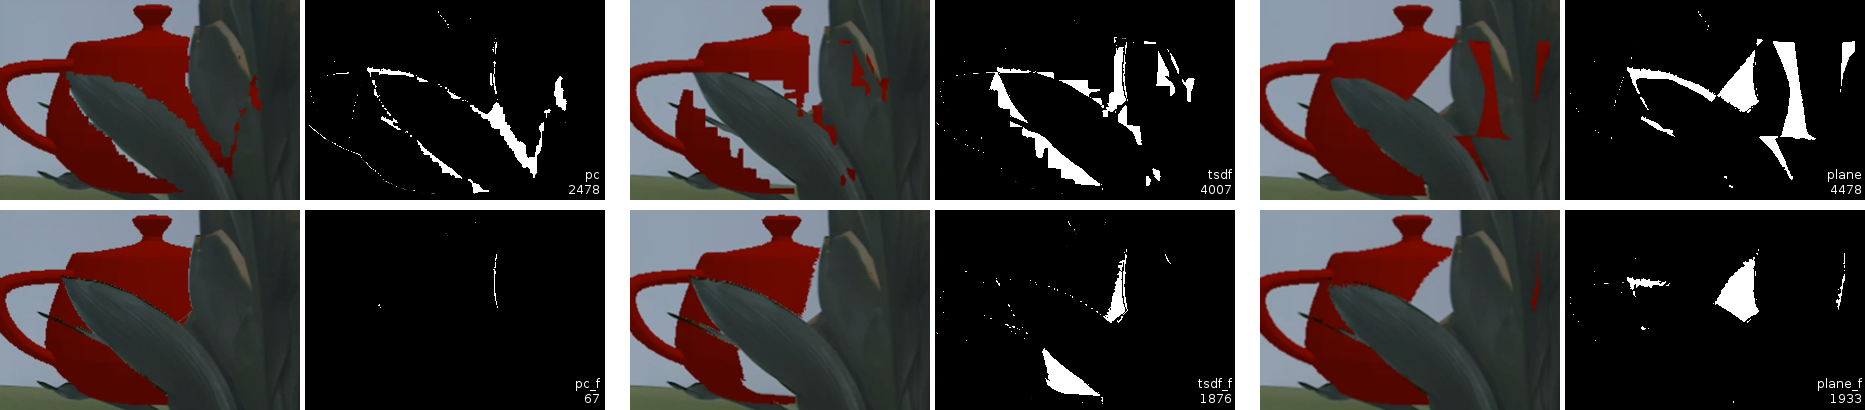
\includegraphics[width=1.0\textwidth]{content/images/evaluation/plant_occlusion_results.png} 
  \caption{Differenzbilder der Verfahren in ersten (oben) und zweiten Szene (unten)}
  \label{fig:static_occlusion_results}
\end{sidewaysfigure}



\addcontentsline{toc}{chapter}{Bibliography}

\bibliography{main}
\bibliographystyle{natdin} 

\end{document}

